\documentclass[11pt]{article}
\pagestyle{plain}
%\documentclass{article}
%\usepackage[utf8]{inputenc}
%\usepackage[english]{babel}

\usepackage{latexsym,amsmath,amssymb}
\usepackage{amsthm}
%\usepackage[notref,notcite]{showkeys}
\usepackage{amsfonts}
\usepackage{geometry}
\usepackage{graphicx}
\usepackage{lmodern}
\usepackage{pifont}
\usepackage{tikz}
\usepackage{pgfplots}
\usepackage{thmtools}
\usepackage{wrapfig}
\usepackage{extarrows}
\usepackage{breqn}
\usepackage{physics}
\usepackage{afterpage}
\usepackage{enumitem}
\usepackage[utf8]{inputenc}
\usepackage{mathrsfs}
\usepackage{scalerel}
\usepackage{stackengine,wasysym}
\usepackage{aligned-overset}
\usepackage{stackengine}
\usepackage{mathtools}
\usepackage{nccmath}
\usepackage{float}
\usepackage{url}
\usepackage{esint}
\graphicspath{ {images/} }

\usepackage{hyperref}
\hypersetup{
    colorlinks = true,
    linkcolor = blue,
    filecolor = magenta,      
    urlcolor = blue,
    citecolor = blue,
}

\urlstyle{same}


\setlength{\oddsidemargin}{1pt}
\setlength{\evensidemargin}{1pt}
\setlength{\marginparwidth}{30pt} % these gain 53pt width
\setlength{\topmargin}{1pt}       % gains 26pt height
\setlength{\headheight}{1pt}      % gains 11pt height
\setlength{\headsep}{1pt}         % gains 24pt height
%\setlength{\footheight}{12 pt} 	  % cannot be changed as number must fit
\setlength{\footskip}{24pt}       % gains 6pt height
\setlength{\textheight}{650pt}    % 528 + 26 + 11 + 24 + 6 + 55 for luck
\setlength{\textwidth}{460pt}     % 360 + 53 + 47 for luck


\theoremstyle{definition}
\newtheorem{problem}{Problem}
\setcounter{problem}{0}
%\numberwithin{problem}{chapter}
\renewcommand\theproblem{\arabic{problem}}

\newtheorem{definition}{Definition}
\newtheorem{theorem}{Theorem}
\newtheorem{corollary}{Corollary}
\newtheorem{lemma}[theorem]{Lemma}
\newtheorem{proposition}{Proposition}
\newtheorem{exercise}{Exercise}[problem]
\newtheorem{remark}{Remark}[problem]
\theoremstyle{definition}
\newtheorem{example}{Example}

\def\dsp{\def\baselinestretch{1.35}\large
\normalsize}
%%%%This makes a double spacing. Use this with 11pt style. If you
%%%%want to use this just insert \dsp after the \begin{document}
%%%%The correct baselinestretch for double spacing is 1.37. However
%%%%you can use different parameter.


\def\U{{\mathcal U}}



\begin{document}


\centerline{\bf Problem Set for Math 1540}
\centerline{Zhen Yao}

\bigskip


\begin{problem}
Prove that the trigonometric polynomials
$$
T(x)=\sum_{k=0}^n a_k\cos kx +\sum_{k=0}^n b_k\sin kx,
\quad a_k,b_k\in\mathbb{R}
$$
form an algebra. {\em Hint:} $\cos x+ i\sin x= e^{ix}$.
\end{problem}
\begin{proof}
With $\cos x+ i\sin x= e^{ix}$, then we can have $\cos kx = \frac{1}{2} \left(e^{ikx} + e^{-ikx}\right)$ and $\sin kx = \frac{1}{2} \left(ie^{-ikx} - ie^{ikx}\right)$. 

Now it suffices to show that $\cos(kx)\sin(lx), \cos(kx)\cos(lx), \sin(kx)\sin(lx)$ are trigonometric polynomials. We have
\begin{align*}
    \cos(kx)\sin(lx) & = \frac{1}{4} \left(e^{ikx} + e^{-ikx}\right) \left(ie^{-ilx} - ie^{ilx}\right) \\
    & = \frac{1}{4} \left(ie^{i(k-l)x} - ie^{i(k+l)x} + ie^{-i(k+l)x} - ie^{i(l-k)x} \right) \\
    & = - \frac{1}{2} \sin((k-l)x) + \frac{1}{2} \sin((k+l)x)
\end{align*}
which is also a trigonometric polynomial. Similarly, $\cos(kx)\cos(lx), \sin(kx)\sin(lx)$ are also trigonometric polynomial. Thus, trigonometric polynomials form an algebra.
\end{proof}

\medskip

\begin{problem}\label{problem_2}
Let $S^1=\{ z\in\mathbb{C}:\, |z|=1\}$ be the unit circle in the complex plane.
Let $\mathcal{A}$ be the algebra of functions of the form
$$
f\left(e^{i\theta}\right)=\sum_{k=0}^N c_k e^{in\theta},
\quad
c_k\in\mathbb{C},\, \theta\in\mathbb{R}.
$$
It is easy to see that
$f\equiv 1$ belongs of $\mathcal{A}$ and $\mathcal{A}$ separates points
(do not prove it).
Prove that there are complex valued functions on $S^1$ that cannot be uniformly approximated by functions in $\mathcal{A}$.
{\em Hint:} For $f\in \mathcal{A}$
$$
\int_0^{2\pi} f\left(e^{i\theta}\right)e^{i\theta}\, d\theta =0\, .
$$
\end{problem}
\begin{proof}
The function $f(z) = z\in \mathcal{A}$ separates points in $S^1$. And we can know that $\frac{1}{z} = e^{-i\theta}$ is not in the closure of $\mathcal{A}$, since
\begin{align*}
    \int^{2\pi}_0 e^{-i\theta} e^{i\theta} d\theta = 2\pi.
\end{align*}
\end{proof}

\begin{remark}
This show that the Stone-Weiestrass theorem holds for real valued functions, but does not hold for complex valued functions.
\end{remark}

\medskip

\begin{proof}[Second Proof of Problem \ref{problem_2}]
Let $f:S^1 \to \mathbb{C}$ and $f\left(e^{i\theta} \right) = \cos \theta = {\rm Re}\, \left(e^{i\theta} \right)$, then we have
\begin{align*}
    \int^{2\pi}_0 f\left(e^{i\theta} \right)e^{i\theta} d\, \theta = \int^{2\pi}_0 \cos \theta (\cos \theta + i \sin \theta) d\, \theta = \pi \neq 0.
\end{align*}
If $g\in \mathcal{A}$, then we have 
\begin{align*}
    \int_0^{2\pi} g\left(e^{i\theta}\right)e^{i\theta}\, d\theta & = \sum^N_{k=0} c_n \int^{2\pi}_0 e^{ik\theta} e^{i\theta} \, d\theta \\
    & = \sum^N_{k=0} c_k \left(\int^{2\pi}_0 \cos(k+1)\theta \, d\theta + i \int^{2\pi}_0 \sin(k+1)\theta \, d\theta \right) \\
    & = 0.
\end{align*}

Now we suppose $\mathcal{A}\ni g_k \rightrightarrows f$, then we have $g_k\left(e^{i\theta}\right) e^{i\theta} \rightrightarrows f\left(e^{i\theta}\right) e^{i\theta}$ and 
\begin{align*}
    0 = \int^{2\pi}_0 g_k\left(e^{i\theta}\right) e^{i\theta} \, d\theta \to \int^{2\pi}_0 f\left(e^{i\theta}\right) e^{i\theta} \, d\theta \neq 0
\end{align*}
which is a contradiction. 
\end{proof}

\medskip


\begin{problem}\label{problem_3}
Prove that complex polynomials
$$
p(z) = \sum_{n=0}^N c_n z^n,
\quad
c_n\in\mathbb{C}
$$
are not dense in $C(\overline{D},\mathbb{C})$, where
$$
\overline{D} = \{ z\in\mathbb{C}:\, |z|\leq 1\}
$$
is the unit disc in $\mathbb{C}$.
{\em Hint:} Consider $f(z)=\overline{z}$. Is the previous exercise
helpful?
\end{problem}
\begin{proof}
For $z = e^{i\theta} = \cos x + i\sin x$, we have $\bar{z} = z^{-1}$. Then, 
\begin{align*}
    \bar{p}(z) = \sum^N_{n=0} \bar{c_n} z^{-n}
\end{align*}
which is not a polynomial, since the exponents are negative.
\end{proof}

\medskip

\begin{proof}[Second Proof of Problem \ref{problem_3}]
Suppose $g_k \rightrightarrows f$, then $g_k\left(e^{i\theta}\right) \rightrightarrows f\left(e^{i\theta}\right)$, where $g_k$ restricted to $S^1 = \{ z\in\mathbb{C}:\, |z|=1\}$ converges uniformly to $f$ which is also restricted to $S^1$. Now we take $f\left(e^{i\theta}\right) = {\rm Re}\,\left(e^{i\theta}\right) = \cos \theta$ and $g_k\left(e^{i\theta}\right) = \sum^N_{n=0}c_n e^{in\theta}$, then we can use the similar argument as second proof of Problem \ref{problem_2}.
\end{proof}

\medskip

\begin{problem}
We know that if $f:[a,b]\to\mathbb{R}$ is continuous and
\begin{align}\label{1}
    \int_a^b f(x)x^n\, dx = 0
\end{align}
for $n=0,1,2,3,\ldots$, then $f(x)=0$ for all $a\leq x\leq b$.
We proved it using the Weierstrass theorem.
Suppose now that $f:[a,b]\to\mathbb{R}$ is continuous and (\ref{1})
holds for all $n\geq 2011$. Does it follow that
$f(x)=0$ for all $a\leq x\leq b$?
\end{problem}
\begin{proof}
Set $g(x) = x^{2011}f(x)$, and then $\int^b_a g(x)x^k dx = 0$ for $k = 0,1,2,\cdot$, which implies $g(x) = 0$. Then, we know that $f(x) = 0$ for all $x\neq 0$.

If $a > 0$, then $f(x) = 0$ on $[a,b]$. If $a\neq 0$, then with continuity of $f$, we have $f(0) = 0$. Thus, $f(x) = 0$ for all $a\leq x\leq b$.
\end{proof}

\medskip

\begin{problem}
Prove that if $f:[0,1]\to\mathbb{R}$ is such that
$$
\int_0^1 f(x) e^{nx}\, dx = 0
\quad
\mbox{for all $n=0,1,2,\ldots$,}
$$
then $f(x)=0$ for all $0\leq x\leq 1$.
Provide two proofs following the methods:
\begin{enumerate}
    \item[(a)] Use the Stone-Weierstrass theorem.
    \item[(b)] Use the change of variables formula and apply
the Weierstrass theorem.
\end{enumerate}
\end{problem}

\begin{proof}
~\begin{enumerate}[label=(\alph*)]
    \item There exists a sequence of the form $p_n(x) = \sum^\infty_{n=0}c_n e^{nx}$ such that converges uniformly to $f(x)$. Since $f$ is continuous on $[0,1]$, hence bounded. Then $\{p_n(x)\}$ is also bounded, and hence $p_n f$ converges uniformly to $f^2$. Then we have
    \begin{align*}
        \int^1_0 f^2(x)\,dx = \lim_{n\to\infty} \int^1_0 p_n(x) f(x)\, dx = 0,
    \end{align*}
    which implies $f(x) = 0, x\in[0,1]$.
    \item Let $e^x = y$, then we have $y = \ln x$, and
    \begin{align*}
        \int_0^1 f(x) e^{nx}\, dx = \int_1^e f(\ln y) y^{n-1}\, dy = 0.
    \end{align*}
    By {\bf Problem 4}, we have $f(\ln y) = 0, y\in[1,e]$, which is equivalent to that $f(x) = 0, x\in[0,1]$.
\end{enumerate}
\end{proof}

\medskip

\begin{problem}
Prove that if $X$ is a compact metric space and $f:X\to X$
is a continuous mapping such that
$$
d(f(x),f(y))<d(x,y)
\quad
\mbox{for all $x,y\in X$},
$$
then there is a fixed point of $f$, i.e. $x\in X$ such that $f(x)=x$.
\end{problem}
\begin{proof}
Define $\alpha = \inf_{x\in X} d(x, f(x))$, since $X$ is compact and $x \mapsto d(x,f(x))$ is continuous, then $\alpha$ is attained. Let $\alpha = d(x_0,f(x_0))$, and we need to prove that $f(x_0) = x_0$.

Suppose if not, i.e., $f(x_0) \neq x_0$, then we have
\begin{align*}
    \alpha \leq d(f(f(x_0)), f(x_0)) < d(f(x_0), x_0) = \alpha
\end{align*}
where we used the fact that $d(f(x),f(y))<d(x,y)$, for all$x,y\in X$. Then this is a contradiction.

It remains to show that there is at most one fixed point. Indeed, if $x_1 \neq x_2$ are two distinct fixed point, then we have $d(x_1, x_2) < d(f(x_1), f(x_2)) = d(x_1, x_2)$, which is a contradiction.
\end{proof}

\medskip

\begin{problem}
Find an example of a function $f:\mathbb{R}\to\mathbb{R}$ such that
$$
|f(x)-f(y)|<|x-y|
\quad
\mbox{for all $x,y\in\mathbb{R}$}
$$
and $f$ has no fixed point. You can find an explicit formula for $f$, but you do not have to. It is enough if you find a convincing argument
that such a function exists. You do not have to be very precise, but your argument has to be convincing.
\end{problem}

\begin{proof}
Take $f(x) = \ln\left(1 + e^x\right)$.
\end{proof}

\medskip


\begin{problem}
Show that there is a unique continuous real valued
function $f:[0,1]\to\mathbb{R}$ such that
$$
f(x) = \sin x + \int_{0}^1 \frac{f(y)}{e^{x+y+1}}\, dy.
$$
\end{problem}
\begin{proof}
Consider the map $T:C([0,1],\mathbb{R})\to C([0,1],\mathbb{R})$ defined by 
\begin{align*}
    T(f)(x) = \sin x + \int^1_0 \frac{f(y)}{e^{x+y+1}}\, dy = f(x).
\end{align*}
Clearly $f$ is a solution to the problem if and only if $T(f) = f$. Since $C([0,1],\mathbb{R})$ is compact, then we only need to show that $T$ is a contraction. Indeed, given $f,h\in C([0,1],\mathbb{R})$, we have
\begin{align*}
    d_\infty(T(f),T(h)) & = \sup_{x\in [0,1]} \left|\int_{0}^1 \frac{f(y)}{e^{x+y+1}}\, dy - \int_{0}^1 \frac{h(y)}{e^{x+y+1}}\, dy \right| \\
    & \leq \sup_{x\in [0,1]} \int^1_0 \frac{\left|f(y) - h(y)\right|}{e^{x+y+1}} \, dy \\
    & \leq d_\infty(f,h) \int^1_0 \frac{1}{e^{x+y+1}} \, dy \\
    & = d_\infty(f,h) (e-1)e^{-x-2}
\end{align*}
and we know that $(e-1)e^{-x-2} < 1$ for $x\in [0,1]$. Thus, $T$ is a contraction.
\end{proof}

\medskip


\begin{problem}
Let $(X,d)$ be a nonempty complete metric space.
Let $S:X\to X$ be a given mapping and write $S^2$ for
$S\circ S$ i.e. $S^2(x)=S(S(x))$. Suppose that $S^2$ is a
contraction. Show that $S$ has a unique fixed point.
\end{problem}
\begin{proof}
Since $S^2$ is conctraction, then there is a unique fixed point of $S^2$, denoted by $x^*$, such that $S^2(x^*) = x^*$. Then we have $S^2(S(x^*)) = S\left(S^2(x^*)\right) = S(x^*)$, which implies that $S(x^*)$ is also a fixed point of $S^2$. Thus, we have $S(x^*) = x^*$, implying $S$ has a unique fixed point.
\end{proof}
\begin{remark}
The statement also holds if $S^n$ is a contraction.
\end{remark}

\medskip

\begin{problem}
Let $E$ be a compact set and
let $\mathcal{F}\subset C(E,\mathbb{R})$ be an equicontinuous family
of functions. Does it imply that the family $\mathcal{F}$
is bounded in $C(E,\mathbb{R})$?
\end{problem}
\begin{proof}
No. We can define $f_n(x) = n, \forall n\in \mathbb{N}, x\in E$. Thus, each $f_n(x), x\in E$ is equicontinuous function, hence $f_n(x) \in \mathcal{F}$. But, $\mathcal{F}$ is not bounded.
\end{proof}

\medskip


\begin{problem}
Let $f:\mathbb{R}^n\to\mathbb{R}$ be bounded and uniformly continuous.
Prove that the family of functions $\{ g_z\}_{z\in\mathbb{R}^n}$,
$g_z(x)=f(x)f(x-z)$ is equicontinuous.
\end{problem}
\begin{proof}
Since $f$ is bounded, then there exists a $M > 0$ such that for all $x\in\mathbb{R}^n$, $|f(x)| \leq M$. Since $f$ is uniformly continuous, then for all $\varepsilon > 0$, there exists $\delta > 0$ such that for all $x,y\in \mathbb{R}^n$, if $d(x,y) < \delta$, $|f(x) - f(y)| < \frac{\varepsilon}{2M}$. Then, for any $z\in \mathbb{R}^n$ we have $d(x-z, y-z) < \delta$, and $|f(x-z) - f(y-z)| < \frac{\varepsilon}{2M}$. Now we have
\begin{align*}
    |f(x)f(x-z) - f(y)f(y-z)| = & |f(x)f(x-z) - f(y)f(x-z) + f(y)f(x-z) \\
    & - f(y)f(y-z)| \\
    \leq & |f(x) - f(y)| \cdot |f(x-z)| + |f(x-z) - f(y-z)| \cdot |f(y)| \\
    \leq &  |f(x-z)| \frac{\varepsilon}{2M} + |f(y)| \frac{\varepsilon}{2M} \leq \varepsilon.
\end{align*}
Hence, for all $\varepsilon > 0$, there exists $\delta > 0$ such that for $\forall x,y$ and $\forall z$, if $d(x,y) < \delta$, then $d(g(x), g(y)) < \varepsilon$. Thus, $\{ g_z\}_{z\in\mathbb{R}^n}$ is equicontinuous.
\end{proof}

\medskip

\begin{problem}
Suppose $E$ is a compact metric space and $f_n:E\to\mathbb{R}$,
$n=1,2,\ldots$ is a bounded and equicontinuous sequence of functions. Suppose that $f_n$ converges pointwise to a continuous
function $f:E\to\mathbb{R}$ (i.e. $f_n(x)\to f(x)$ for every $x\in E$). Prove directly (i.e. without using Arzela-Ascoli theorem)
that $f_n\rightrightarrows f$ uniformly on $E$.
\end{problem}
\begin{proof}
~\begin{enumerate}[label=(\alph*)]
    \item Definition of pointwise convergence is that $f_n$ pointwise converges to $f$ if and only if $\lim_{n\to \infty}f_n(x) = f(x)$ for all $x\in E$, i.e., for any $x\in E$ and $\forall \varepsilon > 0$, there exists $N > 0$, such that for all $n \geq N$, $|f_n(x) - f(x)| < \varepsilon$. Here, the choice of $N$ depends on $x$ and $\varepsilon$.
    \item Definition of uniformly convergence is that for every $\varepsilon > 0$, there exists $N > 0$ such that for all $n\geq N$ and all $x\in E$, $|f_n(x) - f(x)| < \varepsilon$. Here the choice of $N$ works for all $x \in E$.
\end{enumerate}

As $\{f_n\}$ is equicontinuous, there exists a $\delta > 0$, such that for $\forall n \in\mathbb{N}$ and $\forall x,y\in E$:
\begin{align*}
    d(x,y) < \delta \Longrightarrow |f_n(x) - f_n(y)| < \frac{\varepsilon}{3}.
\end{align*}
and letting $n\to \infty$, then the above equation implies
\begin{align*}
    d(x,y) < \delta \Longrightarrow |f(x) - f(y)| < \frac{\varepsilon}{3}.
\end{align*}
Since $E$ is compact, then it can be covered by finite many open balls of radius $\delta$, i.e., there exists a $K > 0$ and $x_1, \cdots, x_K \in E$ such that 
\begin{align*}
    E \subset \bigcup^K_{j=1} B\left(x_j, \delta\right).
\end{align*}
As $f_n$ converges pointwise to $f$, then there exists $N > 0$ such that for $\forall n \geq N$, 
\begin{align*}
    |f_n(x_j) - f(x_j)| < \frac{\varepsilon}{3},
\end{align*}
for all $1\leq j \leq K$.

Now for any $x\in E$, and $\forall n \geq N$, then there exists a $j\in \{1,2,\cdots,K\}$, for which $x\in B(x_j,\delta)$, and hence
\begin{align*}
    |f_n(x) - f(x)| & \leq |f_n(x) - f_n(x_j)| + |f_n(x_j) - f(x_j)| + |f(x_j) - f(x)| \\
    & \leq \frac{\varepsilon}{3} + \frac{\varepsilon}{3} + \frac{\varepsilon}{3} = \varepsilon.
\end{align*}
Thus, $f_n\rightrightarrows f$ uniformly on $E$.
\end{proof}

\medskip

\begin{problem}
Suppose $f_n:\mathbb{R}\to\mathbb{R}$,
$n=1,2,\ldots$ is a bounded and equicontinuous sequence of functions.
Suppose that $f_n$ converges pointwise to a continuous
function $f:\mathbb{R}\to\mathbb{R}$.
Does it imply that
$f_n\rightrightarrows f$ uniformly on $\mathbb{R}$?
\end{problem}
\begin{proof}
No. We can take $f_n(x) = \frac{x}{n}$, which is converges pointwise to $f(x) = 0$, but it does not converges uniformly to $0$. Since for $\varepsilon = 1$, then we cannot find $N > 0$ such that for all $x\in\mathbb{R}$, $\frac{x}{N} < \varepsilon = 1$. 
\end{proof}

\medskip

\begin{problem}
Let $f_n:[a,b]\to\mathbb{R}$ be a sequence
of increasing functions that is pointwise convergent to a
continuous function $f:[a,b]\to\mathbb{R}$. Prove that
$f_n\rightrightarrows f$ uniformly on $[a,b]$.
\end{problem}
\begin{proof}
We want to show that for $\forall \varepsilon > 0$, there exists $N > 0$ such that for $\forall n \geq N$ and $\forall x\in [a,b]$, 
\begin{align*}
    |f_n(x) - f(x)| < \varepsilon.
\end{align*}

Let $g_n(x) = f(x) - f_n(x)$, then $g_n(x)$ is decreasing sequences of continuous functions. Let $\varepsilon > 0$, and 
\begin{align*}
    E_n = \{x\in [a,b]: g_n(x) = f(x) - f_n(x) < \varepsilon\}.
\end{align*}
Then $E_n$ is open since it is the inverse image of continuous function. And we can know that $\{E_n\}$ is an ascending sequence of open sets, since $g_n(x)$ is decreasing and if $x\in E_n$, then $g_n(x) < \varepsilon$ and of course $g_{n+1} < \varepsilon$, which implies $x\in E_{n+1}$. Then we have
\begin{align*}
    E_1\subset E_2\subset \cdots \subset E_n \subset \cdots 
\end{align*}
Now letting $n\to 0$, and we have $g_n(x)\to 0$. Then we will have the sets of $x\in [a,b]$ such that $g_n(x) < \varepsilon$ will be the set $[a,b]$. Then,
\begin{align*}
    [a,b] \subset \bigcup^\infty_{n=1} E_n,
\end{align*}
and since $[a,b]$ is compact, then there exists a finite subcover, such that 
\begin{align*}
    [a,b] \subset \bigcup^N_{n=1} E_n.
\end{align*}

Then for $\varepsilon > 0$ defined above, there exists $N > 0$ such that for all $\forall n \geq N$ and $\forall x\in [a,b]$, $|f_n(x) - f(x)| < \varepsilon$.
\end{proof}

\medskip

Next we present another similar problem regarding the relations between pointwise convergence and uniform convergence.

\begin{exercise}
Let $\{f_n\}$ be an equicontinuous family of functions $f_n: E \to \mathbb{R}$ defined on a compact metric space. Prove that if $f_n$ converges pointewise to a continuous function $f: E \to \mathbb{R}$, then $f_n$ converges uniformly to $f$. Provide a direct argument without using Arzela-Ascoli theorem.
\end{exercise}
\begin{proof}
Since $f$ is continuous and $E$ is compact, then $f$ is uniformly continuous. Equicontinuity of the family $\{f_n\}$ and uniform continuity of $f$ implies that for any $\varepsilon > 0$, there exists $\delta > 0$ such that if for all $x, y \in E$, $d(x,y) < \delta$, then we have
\begin{align*}
    \left|f_n(x) - f_n(y)\right| < \frac{\varepsilon}{3}, \quad \left|f(x) - f(y)\right| < \frac{\varepsilon}{3}.
\end{align*}

Since $E$ is compact, then for open covering $B(x_i, \delta), x_i \in E$, there exists finite subcovering such that $E \subset \bigcup^K_{i=1} B(x_i, \delta)$. Then, for any $x \in E$, there exists some $i = 1, 2, \cdots, K$, such that $x \in B(x_i, \delta)$. Since $f_n$ converges pointwise to $f$, then there exists $N_i > 0$ such that for all $n > N_i$, we have
\begin{align*}
    \left|f_n(x_i) - f(x_i)\right| < \frac{\varepsilon}{3}.
\end{align*}
For the same $\varepsilon$ and $\delta$ above, let $N = \max\{N_i\}$, then for all $n > N$ and any $x \in E$, then there exists $i$ such that $d(x, x_i) < \delta$,
\begin{align*}
    \left|f_n(x) - f(x)\right| & \leq \left|f_n(x) - f_n(x_i)\right| + \left|f_n(x_i) - f(x_i)\right| + \left|f(x_i) - f(x)\right| \\
    & < \frac{\varepsilon}{3} + \frac{\varepsilon}{3} + \frac{\varepsilon}{3} = \varepsilon.
\end{align*}
\end{proof}

\medskip

\begin{problem}
Let  $\{f_n\}$ be a sequence of real valued $C^1$ functions on
$[0,1]$ such that, for all $n$,
$$
|f_n'(x)| \leq \frac{1}{\sqrt{x}}
\ \ (0<x\leq 1),
$$
$$
\int_0^1 f_n(x)\, dx = 0.
$$
Prove that the sequence has a subsequence that converges
uniformly on $[0,1]$.
\end{problem}
\begin{proof}
~\begin{enumerate}[label=(\alph*)]
    \item The second equation implies that there exists $x_n \in [0,1]$ such that $f_n(x_n) = 0$. Also, the first inequality implies
    \begin{align*}
        \left|f_n(x)\right| = \left|\int^{x}_{x_0} f_n'(t)\, dt\right| \leq \left|\int^{x}_{x_0} \frac{1}{\sqrt{t}}\, dt\right| = \left|2\sqrt{t} \Big|^{x}_{x_0} \right| = 2 \left|\sqrt{x} - \sqrt{x_0} \right| \leq 2,
    \end{align*}
    since $x\in [0,1]$. Thus, $f_n$ is bounded. 
    
    \item For $x,y\in [0,1]$ and $|x - y| < \delta = \frac{\varepsilon^2}{4}$, we have 
    \begin{align*}
        \left|f_n(x) - f_n(y)\right| = \left|\int^{x}_{y} f_n'(t)\, dt\right| \leq \left|\int^{x}_{y} \frac{1}{\sqrt{t}}\, dt\right| = 2 \left(\sqrt{y} - \sqrt{x}\right) \leq 2 \sqrt{y - x} < \varepsilon,
    \end{align*}
    where in the last step we used $\sqrt{y} - \sqrt{x} \leq \sqrt{y - x}$, since $\sqrt{y} = \sqrt{y-x+x} \leq \sqrt{y-x} + \sqrt{x}$. Thus, $\{f_n\}$ is equicontinuous.
\end{enumerate}
Hence, the family $\{f_n\}$ is bounded, closed and equicontinuous, then the sequence has a uniformly convergent subsequence.
\end{proof}

\medskip

\begin{problem}
We know that every continuous function $f:[a,b]\to\mathbb{R}$ can be uniformly approximated by polynomials (Weierstrass' theorem). Prove that if
a continuous function $f:\mathbb{R}\to\mathbb{R}$ can be uniformly approximated by polynomials on all of $\mathbb{R}$, then $f$ is a polynomial. 
\end{problem}
\begin{proof}
Suppose that $f$ can be uniformly approximated by polynomial $\{P_n(x)\}$ of degree at most $d$, and the polynomial $P_n(x)$ has the form
\begin{align*}
    P_n(x) = a^d_n x^d + \cdots + a^1_n x + a^0_n
\end{align*}
such that 
\begin{align*}
    \left|f(x) - P_n(x)\right| < \frac{1}{n}, \forall x\in \mathbb{R}.
\end{align*}
Then for any $m,n$, we have
\begin{align*}
    \left|P_n(x) - P_m(x)\right| \leq \left|P_n(x) - f(x)\right| + \left|f(x) - P_m(x)\right| < \frac{1}{n} + \frac{1}{m}
\end{align*}
which implies that $P_n(x) - P_m(x)$ is a polynomial which is bounded on $\mathbb{R}$ and hence a constant. Therefore, there exists some polynomial $P(x)$ and some $c_n \in \mathbb{R}$ such that 
\begin{align*}
    P_n(x) = P(x) + c_n.
\end{align*}
Also, we can have $|c_n - c_m| < \frac{1}{n} + \frac{1}{m}$, which implies $c_n$ is a Cauchy sequence, hence converging to a constant $c$.

Now we claim $f(x) = P(x) + c$. Let $\varepsilon > 0$, and pick $N = \frac{2}{\varepsilon}$, then for $\forall n > N$, we have $|c_n - c| < \frac{\varepsilon}{2}$. Now for $\forall n > N$, we have 
\begin{align*}
    |f(x) - P(x) - c| \leq |f(x) - P_n(x)| + |P_n(x) - P(x) - c| \leq \frac{1}{n} + |c_n - c| = \varepsilon.
\end{align*}
\end{proof}

\medskip

\begin{problem}
Prove that if $f_n:\mathbb{R}\to\mathbb{R}$, $n=1,2,3,\ldots$ are differentiable functions such that
\begin{enumerate}
\item[(a)] $f_n(0)=0$ for all $n$,
\item[(b)] $|f_n'(x)|\leq e^x$ for all $n$ and all $x$, 
\end{enumerate}
then there is a subsequence of $f_n$ that converges pointwise to a continuous function $f:\mathbb{R}\to\mathbb{R}$.\\
{\em Hint:} Show that the family satisfies the assumptions of the Arzela-Ascoli theorem on every interval $[-n,n]$ and then apply the diagonal method.
\end{problem}
\begin{proof}
For any $x\in [-n,n]$, we have 
\begin{align*}
    \frac{|f_n(x) - f_n(0)|}{|x - 0|} = |f'(c)| \leq e^c < e^n,
\end{align*}
where $c\in (0,x)$ or $c\in (x,0)$. Then we have $|f_n(x)| < e^n n$ for all $n$ and $x\in [-n,n]$. Then $\{f_n\}$ is the set of bounded functions. Now we prove that $\{f_n\}$ is equicontinuous on interval $[-n,n]$. For any $\varepsilon > 0$, we pick $\delta = \frac{\varepsilon}{e^n}$. Then for any $x, y\in [-n,n]$, if $|x-y| < \delta$, then
\begin{align*}
    |f(x) - f(y)| = f'(c') |x-y| \leq e^n \frac{\varepsilon}{e^n} = \varepsilon,
\end{align*}
where $c' \in (x,y)$ or $c'\in (y,x)$. Thus, $\{f_n\}$ is equicontinuous. 

For interval $[-1,1]$, $\{f_n\}$ has a convergent subsequence, denoted by $f_{11},f_{12},\cdots$. Now the sequence $\{f_{1n}(x)\}$ is bounded on the interval $[-2,2]$, so it has convergent subsequence, denoted by $f_{21}, f_{22}, \cdots$. Contiune this process and we can have subsequences
\begin{align*}
    f_{11},f_{12},f_{13},\cdots \\
    f_{21},f_{22},f_{23},\cdots \\
    f_{31},f_{32},f_{33},\cdots
\end{align*}
Sequence in each line is a subsequence of the previous one. We now select $f_{11}, f_{22}, f_{33},\cdots$. 

We claim that $\{f_{nn}\}$ is uniformly convergent at every point of $\mathbb{R}$. Let $\varepsilon > 0$, and for any $x\in \mathbb{R}$, there exists $N > 0$, such that $x_i\in [-N,N]$ and $|x - x_i| < \delta$, where $\delta > 0$ as in the definition of equicontinuity. For $n,m \geq N$, we have
\begin{align*}
    \left|f_{nn}(x_i) - f_{mm}(x_i)\right| < \frac{\varepsilon}{3}, x\in [-N, N].
\end{align*}
Then we have
\begin{align*}
    |f_{nn}(x) - f_{mm}(x)| \leq |f_{nn}(x) - f_{nn}(x_i)| + |f_{nn}(x_i) - f_{mm}(x_i)| + |f_{mm}(x_i) - f_{mm}(x)| < \varepsilon.
\end{align*}
Hence $\{f_{nn}(x)\}$ is a Cauchy sequence. Now we define $$f(x) = \lim_{n\to\infty}f_{nn}(x),$$
and we can have
$$|f(x) - f_{nn}(x)| < \varepsilon$$
as $m\to\infty$.
\end{proof}

\medskip

\begin{problem}
Let the functions $f_n:[0,1]\to [0,1]$, $n=1,2,\ldots$,
satisfy $\left|f_n(x)-f_n(y)\right|\leq \left|x-y\right|$ whenever $\left|x-y\right| \geq 1/n$. Prove that the sequence $\{ f_n\}_{n=1}^\infty$ has a uniformly convergent subsequence.
\end{problem}
\begin{proof}
Although functions $f_n$ are not equicontinuous (and not even continuous), one can still apply the Arzela-Ascoli diagonalization argument\cite{1}.

Let $n \in \mathbb{N}$ be fixed. Take any $x_1 \in (0,1)$ and consider the set $U_{x_1}$ defined by
\begin{align*}
    U_{x_1} = \left(x_1 - \frac{2}{n}, x_1 - \frac{1}{n} \right) \bigcup \left(x_1 + \frac{1}{n}, x_1 + \frac{2}{n} \right),
\end{align*}
then $U_{x_1}$ is open and for any $x \in U_{x_1}$, we have $\left|x - x_1\right| > 1/n$, and by the definition of $f_n$, we have
\begin{align*}
    \left| f_n(x) - f_n(x_1) \right| \leq \frac{1}{n}.
\end{align*}
Then, for any $x, y \in [0,1]$ such that $\left|x - x_1\right| \leq 1/n, \left|y - x_1\right| \leq 1/n$, then 
\begin{align*}
    \left| f_n(x) - f_n(y) \right| \leq \left| f_n(x) - f_n(x_1) \right| + \left| f_n(x-1) - f_n(y) \right| \leq \frac{2}{n}.
\end{align*}
Let $x_1$ be arbitrary over $\mathbb{Q}$, then $\{\left(x_1 - 1/n, x_1 + 1/n\right)\}$ will be an open covering of $[0,1]$. Since $[0,1]$ is compact, then there exists a finite subcovering. Then apply above argument on the open set $U_{x_1}$, for any $x, y \in U_x$ or $[0,1] \setminus \left(x_1 - 2/n, x_1 + 2/n\right)$, we have
\begin{align*}
    \left| f_n(x) - f_n(y) \right| \leq \max \left\{ \frac{2}{n}, \left|x - y\right| \right\},
\end{align*}
which shows ‘‘asymptotic equicontinuity’’, the oscillations of $f_n$ decay uniformly as $n \to \infty$.
\end{proof}

\medskip

\begin{problem}
If $f=(f_1,\ldots,f_n):[a,b]\to \mathbb{R}^n$ is a
continuous function, then we define
$$
\int_a^b f(t)\, dt =
\left\langle \int_a^b f_1(t)\, dt, \ldots, \int_a^b f_n(t)\, dt \right\rangle\, .
$$
Prove that
$$
\left\Vert \int_a^b f(t)\, dt \right\Vert \leq
\int_a^b \Vert f(t)\Vert\, dt.
$$
\end{problem}
\begin{proof}
Let $V = (v_1, \cdots, v_n) = \int^b_a f(t)\, dt$, then if $V = 0$, then we are done. If not, by Cauchy Schwarz inequality, we have
\begin{align*}
    \left\|V\right\|^2 & = \sum^n_{i=1} v_i^2 \\
    & = \sum^n_{i=1} v_i \int^b_a f_i(t)\, dt \\
    & = \int^b_a \sum^n_{i=1} \left( v_i f_i(t) \right)\, dt \\
    & \leq \int^b_a \left(\sum v_i^2 \right)^{\frac{1}{2}} \left( \sum f_i(t)^2 \right)^{\frac{1}{2}}\, dt \\
    & = \int^b_a \left\|V\right\| \left\|f(t)\right\|\, dt \\
    & = \left( \int^b_a \left\| f(y) \right\|\, dt \right)^2.
\end{align*}
\end{proof}

\medskip

\begin{problem}
Let $A=\left(a_{ij}\right)_{m\times n}$ be the matrix of a linear mapping
$A\in L(\mathbb{R}^n,\mathbb{R}^m)$. Prove that the norm
$$
\Vert A\Vert=\sup_{\Vert x\Vert=1}\Vert Ax\Vert
$$
satisfies the inequality
$$
\Vert A\Vert \leq\left(\sum_{i=1}^m\sum_{j=1}^na_{ij}^2\right)^{1/2}.
$$
{\em Hint:} You may use the following argument: write the components of the vector $Ax$ as scalar products of rows on $A$ and $x$. Then use the Schwarz inequality to estimate the length of the vector $Ax$.
\end{problem}
\begin{proof}
For $\forall x\in\mathbb{R}^n$, we have
\begin{align*}
    \|Ax\|^2 & = \sum^m_{i=1} \left(\sum^n_{j=1} a_{ij} x_j\right)^2 \\
    & \leq \sum^m_{i=1} \left(\sum^n_{j=1} a_{ij}^2 \right) \left(\sum^n_{j=1} x_{j}^2 \right) \\
    & = \left(\sum_{i=1}^m\sum_{j=1}^na_{ij}^2\right) \|x\|.
\end{align*}
Also, we can have
$$\|A\| = \sup_{\Vert x\Vert=1} \|Ax\| \leq \left(\sum_{i=1}^m\sum_{j=1}^na_{ij}^2\right)^{\frac{1}{2}}.$$
\end{proof}

\medskip

\begin{problem}
Let $f:\mathbb{R}\to\mathbb{R}$ be differentiable and $F:\mathbb{R}^2\to\mathbb{R}$ be defined by
$F(x,y)=f(xy)$. Prove that
$$
x\frac{\partial F}{\partial x}=y\frac{\partial F}{\partial y}\, .
$$
\end{problem}
\begin{proof}
We have $\frac{\partial F}{\partial x} = f'(xy)y$ and $\frac{\partial F}{\partial y} = f'(xy)x$. Thus, we have 
\begin{align*}
    x\frac{\partial F}{\partial x} = y\frac{\partial F}{\partial y} = xy f'(xy).
\end{align*}
\end{proof}

\medskip

\begin{problem}
We say that a function $f:\mathbb{R}^n\to\mathbb{R}$ is homogeneous of degree $m$ if
$f(tx)=t^mf(x)$ for all $x\in\mathbb{R}^n$ and all $t>0$.
Prove that if $f$ is differentiable on $\mathbb{R}^n$ and homogeneous of
degree $m$, then
$$
\sum_{i=1}^n x_i\frac{\partial f}{\partial x_i}(x) = mf(x)
\quad
\mbox{for all $x\in\mathbb{R}^n$.}
$$
\end{problem}
\begin{proof}
Differentiating both sides of the equation $f(tx)=t^mf(x)$ with respect to $t$ and we have
\begin{align*}
    x \cdot \nabla f(tx) = m t^{m-1} f(x).
\end{align*}
Choosing $t = 1$ and we have 
\begin{align*}
    x \cdot \nabla f(x) = \sum^n_{i=1} x_i \frac{\partial f}{\partial x_i}(x) = m f(x).
\end{align*}
\end{proof}

\medskip

\begin{problem}
We know that a function $f(x,y)$ is differentiable at $(0,0)$. We also know the
directional derivatives
$$
\begin{array}{ccc}
D_uf(0,0)=1    & \mbox{where $u=[1/\sqrt{5},2/\sqrt{5}]$,}\\
D_vf(0,0)=1 &   \mbox{where $v=[1/\sqrt{2},1/\sqrt{2}]$}.
\end{array}
$$
Find the gradient $\nabla f(0,0)$.
\end{problem}
\begin{proof}
We have 
\begin{align*}
    \left\{
    \begin{aligned}
        \frac{1}{\sqrt{5}}\frac{\partial f}{\partial x}(0,0) + \frac{2}{\sqrt{5}}\frac{\partial f}{\partial y}(0,0) = 1\\
        \frac{1}{\sqrt{2}}\frac{\partial f}{\partial x}(0,0) + \frac{1}{\sqrt{2}}\frac{\partial f}{\partial y}(0,0) = 1
    \end{aligned}
    \right.
\end{align*}
Then we have $\nabla f(0,0) = \left(\frac{\partial f}{\partial x}(0,0), \frac{\partial f}{\partial y}(0,0) \right) = \left(2\sqrt{2}-\sqrt{5}, \sqrt{5}-\sqrt{2} \right)$.
\end{proof}

\medskip

\begin{problem}
Let $f\in C^1(\mathbb{R}^2)$ be such that $f(1,1)=1$ and $\nabla f(1,1)=(a,b)$.
Let $\varphi(x)=f(x,f(x,f(x,x)))$. Find $\varphi(1)$ and $\varphi'(1)$.
\end{problem}
\begin{proof}
First, we have $\varphi(1) = f(1,f(1,f(1,1))) = f(1,f(1,1)) = f(1,1) = 1$. Second, set $\varphi(x) = f(x, h(x))$, where $h(x) = f(x, f(x,x)) = f(x,g(x))$. Then we have
\begin{align*}
    \varphi'(x) = \partial_1 f(x, h(x)) + \partial_2 f(x, h(x)) h'(x),
\end{align*}
where 
\begin{align*}
    h'(x) & = \partial_1 f(x,g(x)) + \partial_2 f(x,g(x)) g'(x) \\
    g'(x) & = \partial_1 f(x,x) + \partial_2 f(x,x) .
\end{align*}
Then $g'(1) = a+b, g(1) = 1$ and $h'(1) = \partial_1 f(1,1) + \partial_2 f(1,1) (a+b) =a + b(a+b)$. Thus, $\varphi'(1) = a + b (a + b(a+b))$.
\end{proof}

\medskip

\begin{problem}
A function $f:\mathbb{R}^n\to\mathbb{R}$ is differentiable. Find the derivative of the function
$$
F(t)=(f(t,t^2,\ldots,t^n))^2,\quad t\in\mathbb{R}
$$
of one variable.
\end{problem}
\begin{proof}
We have
\begin{align*}
    F'(t) = 2 f(t,t^2,\ldots,t^n) (1 + 2t + \cdots + n t^{n-1}) \frac{\partial f}{\partial t}.
\end{align*}
\end{proof}

\medskip

\begin{problem}
Verify by a direct computation that the vector field $F(x)=x|x|^{-n}$ defined on
$\mathbb{R}^n\setminus\{0\}$ is divergence free, i.e.
$$
{\rm div}\, F(x)=\sum_{i=1}^n \frac{\partial}{\partial x_i}\left(\frac{x_i}{|x|^n}\right) = 0
\quad
\mbox{for all $x\neq 0$.}
$$
\end{problem}
\begin{proof}
\begin{align*}
    {\rm div}\, F(x) & = \sum^n_{i=1} \left(|x|^{-n} - n |x|^{-n-1} x_i^2\right) \\
    & = n |x|^{-n} - n |x|^{-n-2} |x|^2 = 0.
\end{align*}
\end{proof}

\medskip

\begin{problem}
Prove that for $\alpha>0$ the function $\Phi:\mathbb{R}^n\to\mathbb{R}^n$,
$$
\Phi(x)=x|x|^\alpha
$$
is of class $C^1$. Find $D\Phi(x)$.
\end{problem}
\begin{proof}
We need to prove the continuity of $\partial \Phi_i/\partial x_j$, and we have 
\begin{align*}
    \Phi_i (x) = x_j |x|^\alpha \in C^\infty \left( \mathbb{R}^n\setminus \{0\}\right).
\end{align*}
For $x\neq 0$, we have
\begin{align*}
    \frac{\partial \Phi_i(x)}{\partial x_j} & = \frac{\partial x_i}{\partial x_j} |x|^\alpha + x_i \frac{\partial |x|^\alpha}{\partial x_j} \\
    & = \delta_{ij} |x|^\alpha + \alpha x_i x_j |x|^{\alpha - 2} \\
    & = |x|^\alpha \left( \delta_{ij} + \alpha \frac{x_i}{|x|} \frac{x_j}{|x|} \right).
\end{align*}
Some notation are defined as below 
\begin{align*}
    a & = \left[a_1,\cdots,a_n\right]\\
    b & = \left[b_1,\cdots,b_n\right]\\
    a \otimes b & = \begin{pmatrix}
        a_1 b_1 & \cdots &  a_1 b_n\\
        \vdots  & \ddots &  \vdots \\
        a_n b_1 & \cdots & a_n b_n \\
    \end{pmatrix}
\end{align*}
then fr $x\neq 0$, we have 
\begin{align*}
    D\Phi(x) = |x|^\alpha \left( \delta_{ij} + \alpha \frac{x}{|x|} \otimes \frac{x}{|x|} \right),
\end{align*}
and $D\Phi(x) \to 0$ as $x \to 0$. It remains to show that $D\Phi(0) = 0$. 

We prove it directly by definition and we have 
\begin{align*}
    \frac{\Phi(x) - \Phi(0) - 0\cdot x}{|x|} = \frac{x|x|^\alpha}{|x|} = \underbrace{\frac{x}{|x|}}_{\text{bounded}} \cdot |x|^\alpha \xrightarrow{x \to 0} 0.
\end{align*}
Thus, the derivative of $\Phi(x)$ is
\begin{align*}
    D\Phi(x) = \left\{
    \begin{aligned}
        & |x|^\alpha \left( \delta_{ij} + \alpha \frac{x}{|x|} \otimes \frac{x}{|x|} \right), & x \neq 0,\\
        & 0, & x = 0.
    \end{aligned}
    \right.
\end{align*}
\end{proof}

\medskip

\begin{problem}
Find all the points $(x,y)\in\mathbb{R}^2$ where the function
$$
f(x,y)=|e^x-e^y|\cdot(x+y-2)
$$
is differentiable.
\end{problem}
\begin{proof}
~\begin{enumerate}[label=(\arabic*)]
    \item $f$ is $C^\infty$ at $\{(x,y) \in \mathbb{R}^2| x \neq y\}$. Indeed, 
    \begin{align*}
        f(x,y) = \left\{
        \begin{aligned}
            & \left(e^x - e^y\right)(x+y-2), & x > y,\\
            & \left(e^y - e^x\right)(x+y-2), & x < y,
        \end{aligned}
        \right.
    \end{align*}
    is $C^\infty$. 
    
    \item It remains to show the differentiability at point $(x,x)$. We prove it by the definition and we have
    \begin{align*}
        \frac{\partial^+ f}{\partial x}(x,x) & = \lim_{h\to 0^+} \frac{f(x+h,x) - f(x,x)}{h} \\
        & = \lim_{h\to 0^+} \frac{\left(e^{x+h} - e^x\right)(2x+h-2)}{h} \\
        & = \lim_{h\to 0^+} \frac{e^{x+h} - e^x}{h} (2x+h-2) \\
        & = e^x (2x-2), \\
        \frac{\partial^- f}{\partial x}(x,x) & = \lim_{h\to 0^-} \frac{f(x,x+h) - f(x,x)}{h} \\
        & = - e^x (2x-2).
    \end{align*}
    
    Then, when $x\neq 1$,
    \begin{align*}
        \frac{\partial^+ f}{\partial x}(x,x) \neq \frac{\partial^- f}{\partial x}(x,x),
    \end{align*}
    hence, $f$ is not differentiable at $\{(x,x)\}\setminus \{(1,1)\}$.
    
    For the point $(1,1)$, we have 
    \begin{align*}
        \frac{f(1+s,1+t) - f(1,1) - 0\cdot (s,t)}{\sqrt{s^2+t^2}} = \left|e^{1+s} - e^{1+t}\right| \underbrace{\frac{ (s+t)}{\sqrt{s^2+t^2}}}_{\text{bounded}} \xrightarrow{(s,t)\to (0,0)} 0.
    \end{align*}
    Thus, $f$ is differentiable at point $(1,1)$.
\end{enumerate}
\end{proof}


\medskip

\begin{problem}
Consider the function $g : \mathbb{R}^2 \to \mathbb{R}$ given by
$$
g(x, y) = x^{2/3}y^{2/3}, \ \text{for all} \ (x, y) \in \mathbb{R}^2 \,
.
$$
Prove that $g$ is {\it differentiable} at $(0, 0)$.
\end{problem}
\begin{proof}
We have $\frac{\partial g}{\partial x}(0,0) = 0$ and $\frac{\partial g}{\partial y}(0,0) = 0$. Also, we have
\begin{align*}
    \lim_{h\to0} \frac{h^{2/3}h^{2/3}}{h} = 0 = f(0,0).
\end{align*}
Thus, $f$ is continuous at $(0,0)$, hence differentiable at $(0,0)$.
\end{proof}

\medskip

\begin{problem}
Find a function $f:\mathbb{R}^2\to\mathbb{R}$ that is differentiable at each point,
but whose partial derivatives are not continuous at $(0,0)$.
\end{problem}
\begin{proof}
Take 
\begin{align*}
    f(x,y) = \left\{
    \begin{aligned}
        & (x^2 + y^2) \sin \left(\frac{1}{\sqrt{x^2 + y^2}}\right),\, {\rm if }\,\, (x,y)\neq (0,0)\\
        & 0, \, {\rm if }\,\, (x,y) = (0,0)
    \end{aligned}
    \right.
\end{align*}
Then we have 
\begin{align*}
    \frac{\partial f}{\partial x}(0,0) & = \lim_{h\to 0} \frac{f(h,0) - f(0,0)}{h} = \lim_{h\to 0} h \sin \left(1/|h|\right) = 0 \\
    \frac{\partial f}{\partial y}(0,0) & = \lim_{h\to 0} \frac{f(h,0) - f(0,0)}{h} = \lim_{h\to 0} h \sin \left(1/|h|\right) = 0 
\end{align*}
Also, we have
\begin{align*}
    \frac{\partial f}{\partial x}(x,y) & = 2x \sin \left(\frac{1}{\sqrt{x^2 + y^2}}\right) - \frac{x \cos \left(\frac{1}{\sqrt{x^2 + y^2}}\right)}{\sqrt{x^2 + y^2}} \\
    \frac{\partial f}{\partial y}(x,y) & = 2y \sin \left(\frac{1}{\sqrt{x^2 + y^2}}\right) - \frac{y \cos \left(\frac{1}{\sqrt{x^2 + y^2}}\right)}{\sqrt{x^2 + y^2}}
\end{align*}
which oscillate rapidly near the origin. Thus, the partial derivatives are not continuous at $(0,0)$.
\end{proof}

\medskip

\begin{problem}
Prove that the partial derivatives (of first order) of a function
$f:\mathbb{R}^n\to\mathbb{R}$ exist everywhere and they are bounded, then the function $f$ is continuous.
\end{problem}
\begin{proof}
Let $x_0 = (x_{01},\cdots,x_{0n}) \in \mathbb{R}^n$ be arbitray, and define $f_i = \frac{\partial f}{\partial x_i}$. Since partial derivatives exist everywhere and bounded, then we define $M = \sum^n_{i=1}\sup |f_i(x)|, x\in \mathbb{R}^n$. Then, for $x = (x_1,\cdots,x_n)$, we have
\begin{align*}
    |f(x_0) - f(x)| \leq & |f(x_{01},\cdots,x_{0n}) - f(x_1, x_{02}, \cdots, x_{0n})| + \\
    & |f(x_1, x_{02}, \cdots, x_{0n}) - f(x_1, x_{2}, x_{03}, \cdots, x_{0n})| + \cdots  \\
    & + |f(x_{1},\cdots, x_{n-1}, x_{0n}) - f(x_1, \cdots, x_n)| \\
    \leq & M |(x_{01},\cdots,x_{0n}) - (x_1, x_{02}, \cdots, x_{0n})| + \\
    & M |(x_1, x_{02}, \cdots, x_{0n}) - (x_1, x_{2}, x_{03}, \cdots, x_{0n})| + \cdots  \\
    & M |(x_{1},\cdots, x_{n-1}, x_{0n}) - (x_1, \cdots, x_n)|,
\end{align*}
where in the last step we used Mean Value theorem. Thus, we can know that for any $x\in \mathbb{R}^n$, $f(x)$ is bounded.
\end{proof}

\medskip

\begin{problem}
Prove that if $f,g\in C^k(\Omega)$, $\Omega\subset\mathbb{R}^n$, then for any multiindex
$\alpha$ with $|\alpha|\leq k$ we have
$$
D^\alpha(fg)=\sum_{\beta\leq \alpha}\binom{\alpha}{\beta}D^\beta f D^{\alpha-\beta}g\, ,
$$
where
$\beta\leq\alpha$ means that $\beta_i\leq\alpha_i$ for $i=1,2,\ldots,n$,
$\alpha-\beta=(\alpha_1-\beta_1,\ldots,\alpha_n-\beta_n)$ and 
$$
\binom{\alpha}{\beta}=\frac{\alpha!}{\beta!(\alpha-\beta)!}\, .
$$
\end{problem}
\begin{proof}
We have
\begin{align*}
    D^1(fg) & = D^1f g + f D^1 g \\
    D^2(fg) & = D^2f g + D^1 f D^1 g + D^1 f D^1 g + f D^2 g \\
    & \cdots \\
    D^\alpha(fg) & = \sum_{\beta\leq \alpha}\binom{\alpha}{\beta}D^\beta f D^{\alpha-\beta}g,
\end{align*}
where it is like the Binomial theorem.
\end{proof}

\medskip

\begin{problem}
Prove that:
\begin{enumerate}[label=(\alph*)]
    \item There is a unique continuous function $f:[0,1]\to\mathbb{R}$ such that
    $$
    f(x)=1+\int_0^x t^2f(t)\, dt,
    \quad \text{for all $x\in [0,1]$.}
    $$
    \item The function from (a) is of class $f\in C^\infty(0,1)$.
\end{enumerate}
\end{problem}

\begin{proof}
~\begin{enumerate}[label=(\alph*)]
    \item Consider the mapping $T: C([0,1],\mathbb{R})\to C([0,1],\mathbb{R})$ defined by 
    \begin{align*}
        T(f)(x) = g(x) + \int^x_0 t^2 f(t^2)\, dt.
    \end{align*}
    Clearly, $f$ is a solution to the problem if and only if $T(t) = f$. Since $C([0,1],\mathbb{R})$ is compact, then we need to prove that $T(f)$ is a contraction.
    
    Given $f,h \in C([0,1],\mathbb{R})$, we have
    \begin{align*}
        d_\infty(T(f),T(h)) & = \sup_{x\in[0,1]} \left|\int^x_0 t^2 f(t^2)\, dt - \int^x_0 t^2 h(t^2)\, dt\right| \\
        & \leq \sup_{x\in[0,1]} \int^x_0 \left|f(t^2) - h(t^2)\right|t^2\, dt \\
        & \leq d_\infty (f,h) \int^1_0 t^2\, dt = \frac{1}{3} d_\infty (f,h)
    \end{align*}
    which implies that $T$ is a contraction. And the result follows.
    
    \item To prove that $f \in C^\infty(0,1)$, it suffices to show that $k$-th derivative $f^{(k)}$ exists and is continuous on $(0,1)$ for all $k \in \mathbb{N}$. We prove it by induction with respect to $k$.
    
    Note that $f'(x) = x^2 f(x)$ is continuous. Assume now that $f^{(k)}$ exists and is continuous on $(0,1)$, then $x^2f(x)$ is $k$-times differentiable, so is $f'$, which implies $f$ is $(k+1)$-times continuously differentiable.
\end{enumerate}
\end{proof}

\medskip

\begin{problem}
Prove that if $f:\mathbb{R}^n\to\mathbb{R}$ satisfies $\left|f(x) - f(y)\right| \leq M \left|x - y\right|^{3/2}$, then $f$ is constant.
\end{problem}
\begin{proof}
It suffice to show that $Df(x) = 0$ on $\mathbb{R}^n$. By definition, we have 
\begin{align*}
    \frac{\|f(x+h) - f(x) - 0\cdot h\|}{\|h\|} \leq \frac{M \|h\|^{3/2}}{\|h\|} = M \|h\|^{\frac{1}{2}} \xrightarrow[]{h\to\infty} 0,
\end{align*}
which implies $Df(x) = 0$. Hence, $f$ is constant.
\end{proof}


\medskip

\begin{problem}
Prove that if the partial derivatives $\partial f/\partial x_1$ and $\partial f/\partial x_2$  of a function $f:\mathbb{R}^2\to\mathbb{R}$ exist at every point of
$\mathbb{R}^2$, and the partial derivative $\partial f/\partial x_1$ is continuous on $\mathbb{R}^2$, then $f$ is differentiable at every point of $\mathbb{R}^2$.
\end{problem}
\begin{proof}
Let $y = (y_1, y_2), x = (x_1, x_2) \in \mathbb{R}^2$, then we have
\begin{align*}
    f(y_1, y_2) - f(x_1, x_2) & = f(y_1, y_2) - f(x_1, y_2) + f(x_1, y_2) - f(x_1, x_2) \\
    & = \frac{\partial f}{\partial x_1}(\xi, y_2) (y_1 - x_1) + \frac{\partial f}{\partial x_2}(x_1,x_2)(y_2 - x_2) + \varphi(y_2 - x_2)|y_2 - x_2|.
\end{align*}
By definition, we have
\begin{align*}
    & \frac{\left|f(y_1, y_2) - f(x_1, x_2) - \sum^2_{i=1}\frac{\partial f}{\partial x_i}(x_1, x_2)(y_i - x_i) \right|}{\|y - x\|} \\
    \leq & \underbrace{\left|\frac{\partial f}{\partial x_1}(\xi, y_2) - \frac{\partial f}{\partial x_1}(x_1, y_2)\right|}_{\xrightarrow[y\to x]{} 0}\cdot \underbrace{\frac{|y_1 - x_1|}{\|y - x\|}}_{\leq 1} + \underbrace{|\varphi(y_2 - x_2)|}_{\xrightarrow[y\to x]{} 0} \cdot \underbrace{\frac{|y_2 - x_2|}{\|y - x\|}}_{\leq 1} \to 0.
\end{align*}
Hence, $f$ is differentiable at every point of $\mathbb{R}^2$.
\end{proof}

\medskip

\begin{problem}
Prove that if $f\in C^1(\mathbb{R}^n)$ and $\nabla f$ is $L$-Lipschitz, $\Vert \nabla f(x)-\nabla f(y)\Vert\leq L\Vert x-y\Vert$, $x,y\in\mathbb{R}^n$, then
$$
\frac{|f(y)-f(x)-\nabla f(x)(y-x)|}{\Vert y-x\Vert}\leq L\Vert y-x\Vert
\quad
\text{for all $x,y\in\mathbb{R}^n$.}
$$
\end{problem}
\begin{proof}
Since $f\in C^1(\mathbb{R}^n)$, then $f(y) - f(x) = \nabla f(\xi)(y - x)$, where $\xi \in \overline{xy}$. Then we have
\begin{align*}
    LHS & = \frac{\left|\nabla f(\xi)(y - x) - \nabla f(x)(y-x) \right|}{\|y-x\|} \\
    & \leq \| \nabla f(x)-\nabla f(y)\|  \\
    & \leq L \|y-x\|.
\end{align*}
\end{proof}

\medskip

\begin{problem}
Let $f\in C^2(\mathbb{R}^2)$. Suppose that $\nabla f=0$ on a compact set
$E\subset\mathbb{R}^2$. Prove that there is a constant $M>0$ such that
$|f(x)-f(y)|\leq M|x-y|^2$ for all $x,y\in E$. \\
{\em Hint:} Cannot use mean-value theorem here, since $f(y) - f(x) = f'(\xi)(y-x)$ and maybe $\xi \notin E$.
\end{problem}
\begin{proof}
By Problem \ref{problem_38}, we have
\begin{align*}
    f(y) - f(x) & = \nabla f(x)(y-x) + \int^1_0 (1-t) (y-x)^T D^2f(x+t(y-x)) (y-x)\, dt.
\end{align*}
Then we have 
\begin{align*}
    \left|f(y) - f(x)\right| \leq  |y-x|^2 \int^1_0 \left|D^2f(x+t(y-x))\right|\, dt.
\end{align*}
Since $E$ is compact, then $E \subset \overline{B}$, where $\overline{B}$ is a closed ball. And we can set $M = \sup_{\xi \in \overline{B}}\left|D^2 f(\xi)\right|$, then we find the $M$ that satisfies the condition.
\end{proof}

\medskip


\begin{problem}\label{problem_38}
Suppose that $f\in C^2(\mathbb{R}^n)$ has a local minimum at $x=0$ and $f(0)=0$. Prove that for any $x\in\mathbb{R}^n$
$$
f(x)=\int_0^1 (1-t)x^TD^2f(tx)x\, dt,
$$
where $x\in\mathbb{R}^n$ is a column vector and $x^T$ is the horizontal vector.
\end{problem}
\begin{proof}
For any $g\in C^2(\mathbb{R}^n)$, we can derive second order Taylor expansion with integral remainder 
\begin{align*}
    g(1) - g(0) & = \int^1_0 g'(t)\, dt \\
    & = - \int^1_0 g'(t)(1-t)'\, dt \\
    & = -g'(t)(1-t)\Big|^1_0 + \int^1_0 g''(t)(1-t)\, dt \\
    & = g'(0) + \int^1_0 g''(t)(1-t)\, dt, 
\end{align*}
which implies $$g(1) = g(0) + g'(0) + \int^1_0 g''(t)(1-t)\, dt.$$ 

Now we set $g(t) = f(x+t(y-x))$, and we have 
\begin{align*}
    g'(t) & = Df(x+t(y-x)) (y-x) \\
    g''(t) & = (y-x)^T D^2 f(x+t(y-x)) (y-x)
\end{align*}
and then 
\begin{align*}
    f(y) - f(x) = g(1) - g(0) = g'(0) + \int^1_0 g''(t)(1-t)\, dt.
\end{align*}
Hence, we have
\begin{align*}
    f(y) = f(x) + Df(x)(y-x) + \int^1_0 (1-t) (y-x)^T D^2 f(x+t(y-x)) (y-x)\, dt,
\end{align*}
letting $y\to x$ and $x\to 0$, we have
\begin{align*}
    f(x) = \int_0^1 (1-t)x^T D^2f(tx) x\, dt.
\end{align*}
\end{proof}

\medskip

\begin{problem}
We know that $f\in C^2(\mathbb{R})$ is convex if and only if $f''\geq 0$ on $\mathbb{R}$. Prove that $f\in C^2(\mathbb{R}^n)$ is convex if and only if
$H_x(f)=D^2f(x)$ is positive semidefinite for all $x\in\mathbb{R}^n$.
\end{problem}
\begin{proof}
$f$ is convex if and only if its restriction to any line in $\mathbb{R}^n$ is convex. This is equivalent to that $\forall x\in \mathbb{R}^n, \forall v \in \mathbb{R}^n, \|v\| = 1$, $g(t) = f(x+tv)$ is convex. Then we have $g''(t) \geq 0$. Since we have 
\begin{align*}
    g'(t) & = \sum^n_{i=1} \frac{\partial f}{\partial x_i}(x+tv) v_i \\
    g''(t) & = \sum^n_{i=1} \frac{\partial^2 f}{\partial x_i^2}(x+tv) v_i v_j\\
    & = v^T D^2f(x+tv)v,
\end{align*}
then $f$ is convex if and only if $\forall x\in \mathbb{R}^n, \forall v \in \mathbb{R}^n, \|v\| = 1$, $v^T D^2f(x+tv)v \geq 0$. Hence, $D^2f(x) \geq 0, \forall x \in \mathbb{R}^n$.
\end{proof}

\medskip

\begin{problem}
Prove that $x_0\in\mathbb{R}^n$ is a critical point of $f\in C^2(\mathbb{R}^n)$, and $H_{x_0}(f)$ is positive definite, then there are $M>0$ and $\varepsilon>0$ such that
$$
f(x)\geq f(x_0)+M\Vert x-x_0\Vert^2,
\quad \text{whenever $\Vert x-x_0\Vert<\varepsilon$.}
$$
\end{problem}
\begin{proof}
With $Df(x_0) = 0$ and $H_{x_0}(f)$ is positive definite, we have $f$ has local minimum at $x_0$. Then 
\begin{align*}
    f(x) & = f(x_0) + Df(x_0)(x-x_0) + \frac{1}{2} (x-x_0)^T D^2f(\xi) (x-x_0), \xi \in \overline{xy} \\
    & = f(x_0) + \frac{1}{2} (x-x_0)^T D^2f(\xi) (x-x_0),
\end{align*}
and we want to prove $\exists M, \exists \varepsilon, |\xi - x_0| < \varepsilon$ such that $v^T D^2f(\xi)v \geq M\|v\|^2$. 

Suppose not, then there exists $\xi_i \to x_0, \|v_i\| = 1$, such that $v_i^T D^2f(\xi_i)v_i \leq 1/i$. Then we have $D^2f(\xi_i) \to D^2f(x_0)$ as $\xi_i\to x_0$ and hence $D^2f(x_0) \leq 0$, which is a contradiction.
\end{proof}

\medskip

\begin{problem}\label{problem_41}
Let $f:\mathbb{R}^n\to\mathbb{R}$ be a given function. Prove that if there are $M>0$ and $\varepsilon>0$ such that
$$
f(x)\geq f(x_0)+M\Vert x-x_0\Vert,
\quad \text{whenever $\Vert x-x_0\Vert<\varepsilon$,}
$$
then $f$ is not differentiable at $x_0$.
\end{problem}

\begin{proof}
Suppose $f$ is differentiable at $x_0$. $f(x) = f(x_0) + D f(\xi) (x-x_0), \xi \in \overline{x x_0}$. Then let $\xi_i\to x_0$, and we have $D f(\xi_i) \to D f(x_0)$ which is finite. Then, as $x_i\to x_0$, we have 
\begin{align*}
    f(x_i) = f(x_0) + D f(\xi_i)(x_i - x_0) \to f(x_0),
\end{align*}
which is a contraction.
\end{proof}

\medskip

\begin{proof}[Second Proof of Problem \ref{problem_41}]
Suppose to the contrary that $f$ is differentiable at $x_0$. Clearly $x_0$ is a local minimum and hence $\frac{\partial f}{\partial x_i}(x_0) = 0$ for all $i = 1, \cdots, n$. On the other hand, if $|h| < \varepsilon$,
\begin{align*}
    f(x_0 + he_i) \geq f(x_0) + M \left\| (x_0 + he_i) - x_0 \right\| = f(x_0) + M|h|.
\end{align*}
Therefore, for $|h| < \varepsilon$,
\begin{align*}
    \frac{f(x_0 + he_i) - f(x_0)}{|h|} \geq M,
\end{align*}
and hence $\frac{\partial f}{\partial x_i}(x_0) \geq M$, which is a contradiction.
\end{proof}


\medskip

\begin{problem}
Consider an open ball $B=B(a,r)\subset\mathbb{R}^n$. Prove that the function
$$
\varphi(x) = \left\{\begin{array}{ccc}
    \exp\left(\frac{1}{|x-a|^2-r^2}\right)       &  \mbox{if $x\in B$}\, , \\
    0     &  \mbox{if $x\in \mathbb{R}^n\setminus B$}\, ,
    \end{array}
    \right.
$$
in infinitely differentiable on $\mathbb{R}^n$.
\end{problem}

\begin{proof}
Consider the function 
\begin{align*}
    g(x) = \left\{
        \begin{aligned}
        & \exp \left(- \frac{1}{r^2 - |x|^2}\right), x\in B, \\
        & 0, x\in \mathbb{R}^n\setminus B,
        \end{aligned}
    \right.
\end{align*}
And we can know that $g$ is infinitely differentiable everywhere but when $|x| = r^2$. Indeed, for $|x| < r^2$, we have
\begin{align*}
    Dg(x) & = - 2 g(x) \frac{|x|^{1/2}}{(r^2 - |x|^2)^2} \left(x_1,\cdots,x_n \right)
\end{align*}
with induction we can prove that $g^{(k)}(x) = P\left(|x|^{-1}\right)g(x)$, where $P\left(|x|^{-1}\right)$ is a polynomial of $|x|^{-1}$. Thus, $g$ is infinitely differentiable when $|x| \neq r^2$.

Also, by definition, for any $a \in \mathbb{R}^n, |a| = r^2$, we have
\begin{align*}
    Dg(a) = \lim_{h\to 0^-} \frac{g(a - h) - g(a)}{|h|}
\end{align*}
Since $B = B(a,r)\subset\mathbb{R}^n$ is compact in $\mathbb{R}^n$, then with mean-value theorem, we have 
\begin{align*}
    \frac{g(a - h) - g(a)}{|h|} = Dg(\xi),
\end{align*}
and as $h\to 0^-$, $\xi \to a$, and then
\begin{align*}
    Dg(a) = \lim_{h\to 0^-} \frac{g(a - h) - g(a)}{|h|} = \lim_{h\to 0^-} Dg(\xi) = 0.
\end{align*}
Also, by induction we can prove that $D^{(k)}g(a) = 0$, hence $g$ is differentiable everywhere. Now let $f(x) = g(x-a)$, then the proof is complete.
\end{proof}

\medskip

\begin{problem}
A $C^2$ function $f:\mathbb{R}^2\to\mathbb{R}$ is called harmonic if
$$
\frac{\partial^2 f}{\partial x^2} +
\frac{\partial^2 f}{\partial y^2} = 0\, .
$$
Prove that if a harmonic function has a local maximum at $(x_0,y_0)$, then
{\em all} second order partial derivatives of $f$ vanish at $(x_0,y_0)$.
\end{problem}

\begin{proof}
Since $f$ has a local maximum at $(x_0, y_0)$, then its Hessian is negative semidefinite at this point, and when consider it on a vector $v = \begin{pmatrix} 1 \\ 1 \end{pmatrix}$, we have
\begin{align*}
    v^T H_{x_0}(f) v = f_{xx}(x_0,y_0) + f_{yy}(x_0,y_0) + 2 f_{xy}(x_0,y_0) \leq 0.
\end{align*}
Also, with Sylvester's criterion, we have
\begin{align*}
    f_{xx}(x_0,y_0) \leq 0,
\end{align*}
and 
\begin{align*}
    f_{xx}(x_0,y_0) f_{yy}(x_0,y_0) - f^2_{xy}(x_0,y_0) \geq 0.
\end{align*}
Combining these implies that all second order partial derivatives of $f$ vanish at $(x_0,y_0)$.
\end{proof}

\medskip

\begin{problem}
Suppose that a function $f:\mathbb{R}^2\to\mathbb{R}$ of class $C^2$ satisfies the inequality $f_{xx}+f_{yy}\geq 0$ at every point of $\mathbb{R}^2$. Suppose also that all its critical points are non-degenerate, i.e. the matrix of second order derivatives
at the critical point has non-zero determinant. Prove that $f$ cannot have local maximum.
\end{problem}
\begin{proof}
Suppose that $f$ has local maximum at its critical point $x_0$, then we have $f_{xx} < 0$, and $f_{xx}f_{yy} - f_{xy}^2 > 0$, which implies $f_{xx}f_{yy} > 0$ and $f_{yy} < 0$. This is a contradiction with the fact that $f_{xx}+f_{yy}\geq 0$ at every point of $\mathbb{R}^2$.
\end{proof}

\medskip

\begin{problem}
Let $f \in C^2(\Omega) \cap C^0(\overline{\Omega})$, where $\Omega \subset \mathbb{R}^n$ is open and bounded.
Let $\Delta f = \sum_{i=1}^n \partial^2f/\partial x_i^2$ be the Laplace operator.
\begin{enumerate}
    \item[(a)] Show that if for some $\varepsilon > 0$ and $x_0 \in \Omega$ we have $\Delta f(x_0) \geq \varepsilon$, then $f$ has no local maximum at $x_0$.
    
    \item[(b)] Conclude that if $\Delta f(x) \geq \varepsilon$ for some $\varepsilon > 0$ and all $x \in \Omega$, then we have $\sup_{\Omega} f = \sup_{\partial \Omega} f$.
    
    \item[(c)] Conclude that if $\Delta f(x) \geq 0$ for all $x \in \Omega$, then we have $\sup_{\Omega} f = \sup_{\partial \Omega} f$.
\end{enumerate}
{\em Hint for part (c):} Observe that $\Delta |x|^2 = 2n$. Use it to modify a function $f$ in (c) so that you can apply part (b).
\end{problem}

\begin{proof}
~\begin{enumerate}
    \item[(a)] Local maximum requires that $H_{x_0}(f)$ is negative definite, which means the trace $\partial^2f/\partial x_i^2$, $i = 1,2,\cdots,n$ of $H_{x_0}(f)$ are not positive. This is a contradiction with the fact $\Delta f(x_0) \geq \varepsilon$, then $f$ has no local maximum at $x_0$.
    
    \item[(b)] With (a), we can know that $f$ has no local maximum in $\overline{\Omega} \setminus \partial \Omega$. Thus, $\sup_{\Omega} f = \sup_{\partial \Omega} f$.
    
    \item[(c)] Let $f_\varepsilon(x) = f(x) + \varepsilon |x|^2$, then $\Delta f_\varepsilon(x) = \Delta f(x) + 2 \varepsilon n$. Then, we have
    \begin{align*}
        \sup_{\Omega} f(x) \leq \sup_{\Omega} f_\varepsilon(x) \leq \sup_{\partial\Omega} f_\varepsilon(x) \leq \sup_{\partial \Omega} f(x) + 2 \varepsilon n \xrightarrow{\varepsilon \to 0} \sup_{\partial \Omega} f(x).
    \end{align*}
\end{enumerate}
\end{proof}

\medskip

\begin{problem}\label{problem_46}
Let $A=\left(a_{ij}\right)$ be an $n\times n$ matrix. The {\em cofactor} $A_{i,j}$ is the product of $(-1)^{i+j}$ with the $(n-1)\times(n-1)$ determinant of $A$ obtained by deleting the $i$th row and $j$th column in $A$. Prove that
$$
\frac{\partial}{\partial a_{ij}}(\det A)=A_{ij}.
$$
\end{problem}
\begin{proof}
The determinant of $A$ is 
\begin{align*}
    \det A = \sum^n_{i=1} a_{ij} A_{i,j},
\end{align*}
then it follows that
\begin{align*}
    \frac{\partial}{\partial a_{ij}}(\det A)=A_{i,j}.
\end{align*}
\end{proof}

\medskip

\begin{problem}\label{problem_47}
Let $A(t)=\left(x_{ij}(t)\right):(a,b)\to\mathbb{R}^{n\times n}$ be a smooth matrix-valued curve. Prove that if $A(0)=I$, then
$$
\dv{}{t}\Bigg|_{t=0}(\det A(t))=\sum_{i=1}^n x_{ii}'(0)={\rm tr}\, A'(0).
$$
\end{problem}
\begin{proof}
Denote the determinant function of a matrix by $d$ as $\det A = d(r_1, r_2 \cdots, r_n)$, where $r_n$ are rows of $A$. Then we have
\begin{align*}
    \dv{}{t} \det A(t) = d(r_1',r_2,\cdots,r_n) + d(r_1,r_2',\cdots,r_n) + \cdots + d(r_1,\cdots,r_n').
\end{align*}
When $t = 0$, the right hand side become the trace of $A'(0)$. Indeed, the first term $d(r_1',r_2,\cdots,r_n)$ at $t = 0$ will be
\begin{align*}
    \det \begin{pmatrix}
        x_{11}' & x_{12}' & \cdots & x_{1n}' \\
        0       & 1       & \cdots & 0 \\
        \vdots  & \ddots  & \ddots & \vdots \\
        0       & 0       & \cdots & 1
    \end{pmatrix} = x_{11}'(0),
\end{align*}
thus, we have $\dv{}{t}\Big|_{t=0}(\det A(t))=\sum_{i=1}^n x_{ii}'(0)$.
\end{proof}

\medskip

\begin{proof}[Second Proof of Problem \ref{problem_47}]
By Problem \ref{problem_46}, we have for the determinant function $\det: \mathbb{R}^{n^2} \to \mathbb{R}$,
\begin{align*}
    (\nabla \det)(A) = \left[A_{ij}\right]_{n\times n}.
\end{align*}
Then we have 
\begin{align*}
    \dv{}{t} \det A(t) & = (\nabla \det(A))\cdot A'(t) \\
    & =  \underbrace{\left[A_{ij}\right]\cdot \left[x_{ij}'\right]}_{\text{scalar product in $\mathbb{R}^{n^2}$}} \\
    & = \sum^n_{i,j = 1} A_{ij}(t) x_{ij}'(t).
\end{align*}
Also, we have $\left[A_{ij}(0)\right] = \delta_{ij}$, hence 
\begin{align*}
    \dv{}{t}\Bigg|_{t=0}(\det A(t)) = \sum^n_{i,j = 1} \delta_{ij} x_{ij}'(0) = \sum_{i=1}^n x_{ii}'(0).
\end{align*}
\end{proof}


\medskip

\begin{problem}
Let $M_{n\times n}$ denote the vector space of real $n\times n$ matrices.
Define a map $f:M_{n\times n}\to M_{n\times n}$ by $f(X)=X^2$.
Find the derivative of $f$.
\end{problem}
\begin{proof}
We need to find a linear function $L: M^{n \times n} \to M^{n \times n}$ such that 
\begin{align*}
    \lim_{H \to 0} \frac{f(A + H) - F(A) - LH}{\left\| H \right\|} = 0.
\end{align*}
We have $f(A + H) = A^2 + AH + HA + H^2$, and then 
\begin{align*}
    f(A + H) - f(A)= A^2 + AH + HA + H^2.
\end{align*}
Observe that the mapping $L: M_{n\times n}\to M_{n\times n}$, $LH = AH + HA$ is linear and 
\begin{align*}
    \left|\frac{f(A + H) - F(A) - LH}{\left\| H \right\|} \right| = \left| \frac{H^2}{\left\| H \right\|} \right| \leq \frac{\left\| H \right\|^2}{\left\| H \right\|} = \left\| H \right\| \xrightarrow{H \to 0} 0, 
\end{align*}
and thus $Df(A): M_{n\times n}\to M_{n\times n}$ is defined by $Df(A)H = AH + HA$.
\end{proof}

\medskip

\begin{problem}\label{problem_49}
The class of invertible matrices
$GL(n,\mathbb{R})$ forms an open subset in the space of all $n\times n$ matrices $M_{n\times n}=\mathbb{R}^{n^2}$.
Let $F:GL(n,\mathbb{R})\to GL(n,\mathbb{R})$, $F(A)=A^{-1}$.
Prove that the function $F$ is $C^\infty$ smooth (as a mapping from $\mathbb{R}^{n^2}$ to $\mathbb{R}^{n^2}$) and that
for any $A\in\mathbb{R}^{n\times n}$ we have
$$
DF(A)B=-A^{-1} B A^{-1},
\quad \text{for all $B\in \mathbb{R}^{n\times n}$}.
$$
\end{problem}
\begin{proof}
Since $AA^{-1} = I$, then $A' A^{-1} + A \left(A^{-1}\right)' = 0$. Thus, $DF(A) = \left(A^{-1}\right)' = - A^{-1} A' A^{-1}$. We can prove by induction that $F(A)$ is infinitely differentiable.

For any $B \in \mathbb{R}^{n\times n}$, we can have 
\begin{align*}
    F(A+B) - F(A) & = \left(A+B\right)^{-1} - A^{-1} \\
    & = \left(A \left(I+A^{-1}B \right) \right)^{-1} - A^{-1} \\
    & = \left(\left(I+A^{-1}B \right) - I \right) A^{-1},
\end{align*}
Then, for $B$ small enough, we have
\begin{align*}
    F(A+B) - F(A) - \left(- A^{-1} B A^{-1}\right) & = \left(\left(I+A^{-1}B \right) - I + A^{-1} B\right) A^{-1} \\
    & = \left(\sum^\infty_{k=0}(-1)^k \left(A^{-1}B\right)^k  - I + A^{-1} B\right) A^{-1} \\
    & = \sum^\infty_{k=2}(-1)^k \left(A^{-1}B\right)^k A^{-1} \to 0.
\end{align*}
Hence, $DF(A)B = -A^{-1} B A^{-1}$.
\end{proof}

\medskip

\begin{proof}[Second Proof of Problem \ref{problem_49}]
The formula for the inverse matrix $A^{-1} = \operatorname{adj}(A) / A^{-1}$ shows that the entries of $F(A) = A^{-1}$ are rational functions rational functions of entries of $A$ with the dinominator $\det A \neq 0$, so $F \in C^\infty$.

Let $G(A) = A$. Since $G$ is the identity mapping, then $DG(A) = I$, i.e., $DF(A)B = B$. Since we have
\begin{align*}
    (F \cdot G)(A) = A^{-1} A = I,
\end{align*}
then $F \cdot G: M^{n \times n} \to M^{n \times n}$ is a constant function, and hence $D(F \cdot G)(A) = 0$, which also implies that $D(F \cdot G)(A)B = 0$ for all $B \in M^{n \times n}$. Applying the chain rule\footnote{Given two differentiable matrix functions $F, G: M^{n \times n} \to M^{n \times n}$, then we have 
$$D(F\cdot G)(A)B = \left(DF(A)B \right)\cdot G(A) + F(A) \cdot \left(DG(A)B \right).$$
Indeed, the result follows from the following argument
\begin{align*}
    (F\cdot G)(A+H) & = F(A+H)\cdot G(A+H) \\
    & = \left(F(A) + DF(A)H + o(H)\right) \left(G(A) + DG(A)H + o(H)\right) \\
    & = \underbrace{F(A)G(A)}_{(F\cdot G)(A)} + \underbrace{\left( (DF(A)H)\cdot G(A) + F(A) \cdot DG(A)H  \right)}_{D(F\cdot G)(A)H} + o(H).
\end{align*}} gives
\begin{align*}
    0 & = D(F \cdot G)(A)B \\
    & = \left( DF(A)B \right) G(A) + F(A) \left( DG(A)B \right) \\
    & = \left( DF(A)B \right) A^{-1} + A^{-1} H,
\end{align*}
and thus, we have $DF(A)B = - A^{-1}BA^{-1}$.
\end{proof}

\begin{problem}
Let $f:\mathbb{R}^n\to\mathbb{R}$ be convex. Prove that if partial derivatives
$$
\frac{\partial f}{\partial x_i}(x_0),
\quad i=1,2,\ldots,n,
$$
exist, then $f$ is differentiable at $x_0$.
\end{problem}
\begin{proof}
Let $A = \left[\frac{\partial f}{\partial x_1}(x_0), \cdots, \frac{\partial f}{\partial x_n}(x_0)\right]$, and we need to prove that 
\begin{align*}
    \phi(h) = f(x_0+h) - f(x_0) - Ah
\end{align*}
satisfies $\frac{\phi(h)}{\|h\|} \to 0$ as $h \to 0$. Note that $\phi(h)$ is convex\footnote{Indeed, for $h_1, h_2 \in \mathbb{R}^n$ and $t \in (0,1)$, by convexity of $f$, we have
\begin{align*}
    \phi(th_1 + (1-t)h_2) & = f(x_0 + th_1 + (1-t)h_2) - f(x_0) \\
    & = f(t(x_0+h_1) + (1-t)(x_0+h_2)) - f(x_0) \\
    & \leq t \left(f(x_0+h_1) - f(x_0) \right) + (1-t) \left(f(x_0+h_2) - f(x_0) \right) \\
    & = t\phi(h_1) + (1-t)\phi(h_2).
\end{align*}} and we denote by $h = \left(h_1, \cdots, h_n \right) = e_1 h_1 + \cdots + e_n h_n$, then we have 
\begin{align*}
    \phi(h) & = \phi \left(\frac{1}{n} \sum^n_{i=1} h_i n e_i \right) \\
    & \leq \frac{1}{n}\sum^n_{i=1} h_i n e_i = \sum^n_{i=1} h_i \frac{\phi(h_i n e_i)}{h_i n} \\
    & \leq \|h\| \sum^n_{i=1} \left|\frac{\phi(h_i n e_i)}{h_i n}\right|,
\end{align*}
similarly, 
\begin{align*}
    \phi(-h) \leq \|h\| \sum^n_{i=1} \left|\frac{\phi( - h_i n e_i)}{ - h_i n}\right|.
\end{align*}
Also, we have $0 = \phi \left(\frac{h + (-h)}{2}\right) \leq \frac{\phi(h) + \phi(-h)}{2}$, which implies $\phi(h) \leq - \phi(-h)$, then 
\begin{align*}
    0 \xleftarrow{h \to 0} - \sum^n_{i=1} \left|\frac{\phi( - h_i n e_i)}{ - h_i n}\right| \leq \frac{\phi(h)}{\|h\|} \leq \sum^n_{i=1} \left|\frac{\phi( h_i n e_i)}{ h_i n}\right| \xrightarrow{h \to 0} 0,
\end{align*}
where in the last step we used the fact that partial derivatives $\frac{\partial f}{\partial x_i}(x_0), i=1,2,\ldots,n$ exist, also we have $\phi(t e_i) = f(x_0+t e_i) - f(x_0) - \frac{\partial f}{\partial x_i}(x_0)t$ and 
\begin{align*}
    \lim_{t\to 0}\frac{\phi(t e_i)}{t} = \lim_{t\to 0} \frac{f(x_0+t e_i) - f(x_0)}{t} - \frac{\partial f}{\partial x_i}(x_0) = 0,
\end{align*}
which together implies $\frac{\phi(h)}{\|h\|} \to 0$.
\end{proof}

\medskip

\begin{problem}
Let $Q:C^\infty(\mathbb{R}^n)\to\mathbb{R}$ be a linear mapping such that $Qf\geq 0$ whenever $f\in C^\infty(\mathbb{R}^n)$ satisfies $f(0)=0$ and $f(x)\geq 0$ in a neighborhood of $0$. Prove that there are real numbers $a_{ij}$, $b_i$ and $c$ such that
$$
Qf=\sum_{i,j=1}^n a_{ij}\frac{\partial^2 f}{\partial x_i\partial x_j}(0)+\sum_{i=1}^n b_i\frac{\partial f}{\partial x_i}(0)+cf(0)
\quad
\text{for all $f\in C^\infty(\mathbb{R}^n)$.}
$$
\end{problem}
\begin{proof}
We have 
\begin{align*}
    f(x) = f(0) + \sum^n_{i=1} \frac{\partial f}{\partial x_i}(0) x_i + \frac{1}{2} \sum_{i,j} \frac{\partial^2 f}{\partial x_i \partial x_j}(0) x_i x_j + \varphi(x),
\end{align*}
and let $c = Q(0), b_i = Q(x_i), a_{ij} = \frac{1}{2}Q(x_i x_j)$, then we have 
\begin{align*}
    Qf = \sum_{i,j=1}^n a_{ij}\frac{\partial^2 f}{\partial x_i\partial x_j}(0) + \sum_{i=1}^n b_i\frac{\partial f}{\partial x_i}(0) + cf(0) + Q\varphi.
\end{align*}
We need to prove that $Q\varphi = 0$. Since $\varphi(x) = o(|x|^2)$, then there exists $\varepsilon > 0$, such that $\varepsilon |x|^2 - \varphi(x) \geq 0$ near $0$. Then, $Q \left(\varepsilon |x|^2 - \varphi(x) \right) \geq 0$, which implies $Q\varphi \leq \varepsilon Q\left(|x|^2\right)$, and then $Q\varphi \leq 0$ as $\varepsilon \to 0$. Similarly, $Q \left(\varepsilon |x|^2 + \varphi(x) \right) \geq 0$ and we have $-Q\varphi \leq \varepsilon Q \left(|x|^2\right)$. Then, $Q\varphi \geq 0$ and hence $Q\varphi = 0$.
\end{proof}

\medskip

\begin{problem}
Define $f:\mathbb{R}^2\to\mathbb{R}$ by
$$
f(x)=
\begin{cases}
\frac{x^2(y^4+2x)}{x^2+y^4}, & \text{if $(x,y)\neq (0,0)$,}\\
0,                           & \text{if $(x,y)=(0,0)$.}
\end{cases}
$$
Prove that $f$ is differentiable at $(0,0)$.
\end{problem}
\begin{proof}
We have 
\begin{align*}
    f_x(0,0) & = \lim_{s\to 0} \frac{f(s,0) - f(0,0)}{s} = \lim_{s\to 0} \frac{2s^3/s^2}{s} = 2 \\
    f_y(0,0) & = \lim_{s\to 0} \frac{f(0,s) - f(0,0)}{s} = 0
\end{align*}
and we need to show that the limit equals zero, which is 
\begin{align*}
    & \lim_{(s,t)\to (0,0)} \frac{f(s,t) - f(0,0) - f_x(0,0)s - f_y(0,0)t}{\sqrt{s^2 + t^2}} \\
    = & \lim_{(s,t)\to (0,0)} \frac{s^2 t^4 - 2s t^4}{(s^2+t^4)\sqrt{s^2 + t^2}},
\end{align*}
also,
\begin{align*}
    \left|\frac{s^2 t^4 - 2s t^4}{(s^2+t^4)\sqrt{s^2 + t^2}}\right| \leq \left|\frac{s^2 t^4 - 2s t^4}{2 |s| t^2 |t|}\right| = \left| \frac{|st|}{2} - t \right| \xrightarrow{(s,t)\to (0,0)} 0,
\end{align*}
where we used the fact that $s^2 + t^4 \geq 2|s|t^2$ and $\sqrt{s^2 + t^2} \geq |t|$.
\end{proof}

\medskip

\begin{problem}
Let $f:\mathbb{R}^2\to\mathbb{R}$ be defined by
$$
f(x)=
\begin{cases}
xy\frac{x^2-y^2}{x^2+y^2}, & \text{if $(x,y)\neq (0,0)$,}\\
0,                           & \text{if $(x,y)=(0,0)$.}
\end{cases}
$$
Prove that the mixed partial derivatives
$\frac{\partial^2 f}{\partial x\partial y}$ and
$\frac{\partial^2 f}{\partial y\partial x}$
exist everywhere in $\mathbb{R}^2$, but
$$
\frac{\partial^2 f}{\partial x\partial y}(0,0)\neq
\frac{\partial^2 f}{\partial y\partial x}(0,0).
$$
\end{problem}
\begin{proof}
When $(x,y) \neq (0,0)$, with $f(x,y) = - f(y,x)$
\begin{align*}
    \frac{\partial f}{\partial x}(x,y) & = \frac{y(x^4 + 4x^2y^2 - y^4)}{\left(x^2 + y^2\right)^2}\\
    \frac{\partial f}{\partial y}(x,y) & = - \frac{\partial f}{\partial x}(y,x) = - \frac{y(x^4 + 4x^2y^2 - y^4)}{\left(x^2 + y^2\right)^2},
\end{align*}
then $\frac{\partial^2 f}{\partial x\partial y}, \frac{\partial^2 f}{\partial y\partial x}$ exist at $(x,y) \neq (0,0)$. Also, 
\begin{align*}
    \frac{\partial^2 f}{\partial y \partial x}(0,0) & = \frac{\partial}{\partial y}\left(\frac{\partial f}{\partial x}\right)(0,0) = \dv{}{y}\Bigg|_{y=0} \left(\frac{\partial f}{\partial x}(0,y)\right) = \dv{}{y}\Bigg|_{y=0} \left(- \frac{y^5}{y^4}\right) = -1, \\
    \frac{\partial^2 f}{\partial x\partial y}(0,0) & = \frac{\partial}{\partial x}\left(\frac{\partial f}{\partial y}\right)(0,0) = \dv{}{x}\Bigg|_{x=0} \left(\frac{\partial f}{\partial y}(x,0)\right) = \dv{}{x}\Bigg|_{x=0} \left(\frac{x^5}{x^4}\right) = 1.
\end{align*}
\end{proof}

\medskip

\begin{problem}
Prove that the function
$$
f(x)=
\begin{cases}
\frac{x|y|}{\sqrt{x^2+y^2}}, & \text{if $(x,y)\neq (0,0)$,}\\
0,                           & \text{if $(x,y)=(0,0)$.}
\end{cases}
$$
has all directional derivatives $D_vf(0,0)$ at the origin, but $f$ is not differentiable at $(0,0)$.
\end{problem}
\begin{proof}
For $v = (a,b) \neq (0,0)$, 
\begin{align*}
    D_vf(0,0) & = \lim_{t\to 0} \frac{f(ta,tb) - f(0,0)}{t} \\ 
    & = \lim_{t\to 0} \frac{1}{t} \frac{ta|tb|}{|t|\sqrt{a^2+b^2}} \\
    & = \lim_{t\to 0} \frac{a|b|}{\sqrt{a^2+b^2}},
\end{align*}
and $D_vf(0,0)$ is not linear with respect to $v$, thus, not differentiable.
\end{proof}

\medskip

\begin{problem}\label{problem_55}
Let $f:\mathbb{R}^n\to\mathbb{R}^n$ be a mapping of class $C^1$. Prove that if $\operatorname{rank} Df(x_0)=n$, then $f$ is injective(one-to-one) in a neighborhood of $x_0$. Prove it directly, without using the inverse function theorem.
\end{problem}
\begin{proof}
Since $\operatorname{rank} Df(x_0) = n$, then $M = f^{-1}(0) = \{x \in \mathbb{R}^n | f(x) = 0\}$ is $0$-dimensional manifold. Thus, $M = \{0\}$, which implies $f$ is injective.
\end{proof}

\medskip

\begin{proof}[Correct Proof of Problem \ref{problem_55}]
Suppose to the contrary that $f$ is not injective in any neighborhood of $x_0$, that is, for any $\varepsilon > 0$, there exist $x, y \in B(x_0, \varepsilon), x\neq y$ such that $f(x) = f(y)$. Take $\varepsilon = 1/n$, and we can find $x_n, y_n \in B(x_0, 1/n), x_n \neq y_n$ such that $f(x_n) = f(y_n)$. Then we have
\begin{align*}
    f(x_n) - f(y_n) = Df(\xi_n) (y_n - x_n), \xi \in \overline{x_ny_n},
\end{align*}
which implies $Df(\xi_n)v_n = 0$, $v_n = \frac{y_n - x_n}{\|y_n - x_n\|}$. By compactness of the unit sphere, we could take a subsequence $\left\{v_{n_k} \right\}$ of $\{v_n\}$ such that $\lim_{k\to\infty} v_{n_k} = v, \|v\| = 1$. Note that $\xi \to x_0$, and hence
\begin{align*}
    0 = Df(\xi_{n_k}) v_{n_k} \to Df(x_0)v,
\end{align*}
which contradicts the fact that $\rank Df(x_0) = 0$.
\end{proof}

\medskip

\begin{problem}
Assume that $f:\mathbb{R}^n\to\mathbb{R}^m$ is differentiable and $\operatorname{rank} Df(x)=n$ for all $x\in\mathbb{R}^n$. Prove that if $S\subset\mathbb{R}^n$ is bounded, then for every $y\in\mathbb{R}^m$, the set $S\cap f^{-1}(y) = \{x\in S: \, f(x) = y\}$ is finite.
\end{problem}
\begin{proof}
Suppose to the contrary that there is $y \in \mathbb{R}^m$ such that $S\cap f^{-1}(y)$ is infinite. Let $\{x_n\}$ be an infinite subset of $S\cap f^{-1}(y)$, and $x_i \neq x_j$ for $i \neq j$. Since $\{x_n\}$ is a bounded, then it has a convergent subsequence $\left\{x_{n_k} \right\} \in S\cap f^{-1}(y)$ such that $\lim_{k \to \infty} x_{n_k} = x_0$. Since $x_{n_k} \in f^{-1}(y)$ and $f^{-1}(y)$ is closed, then we can conclude that $x_0 \in f^{-1}(y)$, that is
\begin{align*}
    f\left(x_{n_k}\right) = f(x_0) = y.
\end{align*}

Since $x_i \neq x_j$ for $i \neq j$, we could further require that $x_{n_k} \neq x_0$ for all $k$. Let $v_k = \frac{x_{n_k} - x_0}{\left\|x_{n_k} - x_0\right\|}$, and since it is a bounded sequence in a compact unit sphere, it has a convergent subsequence $\left\{v_{j_l}\right\}$ such that $\lim_{j\to\infty} v_{j_l} = v_0$, $\|v_0\| = 1$. Since $f$ is differentiable, then 
\begin{align*}
    0 & = \lim_{l\to\infty} \frac{f\left(x_{n_{k_l}}\right) - f(x_0) - Df(x_0)\left(x_{n_{k_l}} - x_0\right)}{\left\| x_{n_{k_l}} - x_0 \right\|} \\
    & = \lim_{l\to\infty} - Df(x_0) \frac{x_{n_{k_l}} - x_0}{\left\| x_{n_{k_l}} - x_0 \right\|} = - Df(x_0) v_0,
\end{align*}
which contracdicts the fact that $\rank Df(x_0) = n$.
\end{proof}
\begin{remark}
Since we do not assume continuity of $Df$, we cannot use the inverse function theorem.
\end{remark}

\medskip

\begin{problem}
Let $\Omega=\{(x,y)\in\mathbb{R}^2:\, x>0, 0<y<2\pi\}$.
Prove that the mapping $f:\Omega\to\mathbb{R}^2$,
$f(x,y)=(x\cos y,x\sin y)$ is a diffeomorphism of $\Omega$
onto an open subset of $\mathbb{R}^2$. Find $f(\Omega)$.\\
{\em Hint:} A picture will help. Have you seen a similar mapping in Calculus~3?
\end{problem}
\begin{proof}
~\begin{enumerate}[label=(\alph*)]
    \item Since
    \begin{align*}
        Jf(x) = \det \begin{pmatrix}
            \cos y & -x \sin y \\
            \sin y & -x \cos y
        \end{pmatrix} = x \neq 0,
    \end{align*}
    the mapping $f$ is diffeomorphism and hence invertible in a neighborhood of any point $(x,y) \in \mathbb{R}^2$. Suppose $f(x_1, y_1) = f(x_2, y_2)$, then we have
    \begin{align*}
        x_1 \cos y_1 & = x_2 \sin y_2 \\
        x_1 \sin y_1 & = x_2 \sin y_2
    \end{align*}
    which implies $x_1 = x_2$ and $y_1 = y_2$. Thus, $f$ is invertible and one-to-one form $\mathbb{R}^2$ to $f(\mathbb{R}^2)$, ane hence $f$ is diffeomorphism of $\Omega$ onto an open subset $f(\mathbb{R}^2)$.
    
    \item $f(\Omega) = \mathbb{R}^2\setminus \{(x, y) \in \mathbb{R}^2 \,|\, x > 0, y = 0\}$.
\end{enumerate}

\end{proof}

\medskip

\begin{problem}
Find a diffeomorphism of $\mathbb{R}^2$ onto the open unit disc $x^2 + y^2 < 1$.
\end{problem}
\begin{proof}
$f(x,y) = \left(\frac{x}{\sqrt{x^2+y^2}+1}, \frac{y}{\sqrt{x^2+y^2}+1}\right)$.
\end{proof}

\medskip

\begin{problem}
Find a diffeomorphism of the upper half plane $y>0$ onto the first quadrant $x>0$, $y>0$.
\end{problem}
\begin{proof}
$f(x,y) = \left(e^x, y\right)$.
\end{proof}

\medskip

\begin{problem}
Suppose that $f\in C^1(\mathbb{R})$ is such that $|f'(x)|<1$ for all $x\in\mathbb{R}$. Prove that the mapping $F:\mathbb{R}^2\to\mathbb{R}^2$,
$F(x,y)=(x+f(y), y-f(x))$ is a diffeomorphism in a neighborhood of any point $(x,y)\in\mathbb{R}^2$.
\end{problem}
\begin{proof}
Since
\begin{align*}
    JF(x) = \det \begin{pmatrix}
        1 & f'(y) \\
        - f'(x) & 1
    \end{pmatrix} = 1 + f'(x)f'(y) \neq 0,
\end{align*}
the mapping $F$ is diffeomorphism and hence invertible in a neighborhood of any point $(x,y) \in \mathbb{R}^2$
\end{proof}

\medskip

\begin{problem}
Prove that a complex polynomial
$P(z)=a_0z^n+a_1 z^{n-1} + \ldots + a_n$
regarded as a function $P:\mathbb{R}^2\to\mathbb{R}^2$ is a diffeomorphism in a neighborhood of $z_0\in\mathbb{C}$
if and only if $P'(z_0)\neq 0$, where
$P'(z)=na_0 z^{n-1} + (n-1)a_1 z^{n-2} + \ldots + a_1$.
\end{problem}
\begin{proof}
~\begin{enumerate}[label=(\alph*)]
    \item If $P$ is a diffeomorphism in a neighborhood of $z_0 = x_0 + i y_0 \in\mathbb{C}$, we can write $P$ as $P(z_0) = u(x_0, y_0) + i v(x_0, y_0)$, where $u,v$ are real functions. Then, with the Cauchy-Riemann equations $u_x = v_y, u_y = -v_x$, we have
    \begin{align*}
        JP(z_0) & = \det \begin{pmatrix}
        u_x(z_0) & u_y(z_0) \\
        v_x(z_0) & v_y(z_0)
        \end{pmatrix} \\
        & = u_x(z_0) v_y(z_0) - u_y(z_0) v_x(z_0) \\
        & = u_x^2(z_0) + u_y^2(z_0) = v_x^2(z_0) + v_y^2(z_0) \neq 0,
    \end{align*}
    which implies $u_x, u_y, v_x, v_y \neq 0$. Also, with Wirtinger derivatives, we have 
    \begin{align*}
        \frac{\partial P}{\partial z} &= \frac12\left(\frac{\partial P}{\partial x} - i\frac{\partial P}{\partial y}\right)\\
        &= \frac12\left(u_x+iv_x - i(u_y+iv_y)\right)\\
        &= \frac12\left((u_x+v_y) + i(v_x-u_y)\right)\\
        &= u_x + iv_x,
    \end{align*}
    and then $P'(z_0) \neq 0$.
    
    \item If $P'(z_0) \neq 0$, then so are $u_x(z_0), v_x(z_0)$. Thus, $JP(z_0) \neq 0$, which implies $P$ is a diffeomorphism in a neighborhood of $z_0 \in\mathbb{C}$.
\end{enumerate}
\end{proof}

\medskip

\begin{problem}
Let $f:\mathbb{R}\to\mathbb{R}$ be $C^1$ and let
\begin{eqnarray*}
u & = & f(x), \\
v & = & -y+xf(x).
\end{eqnarray*}
If $f'(x_0)\neq 0$, show that this transformation is locally
invertible near $(x_0,y_0)$ and the inverse has the form
\begin{eqnarray*}
x & = & g(u), \\
y & = & -v+ug(u).
\end{eqnarray*}
\end{problem}
\begin{proof}
Since 
\begin{align*}
    \det \begin{pmatrix}
        u_x & u_y \\
        v_x & v_y
    \end{pmatrix} = - f'(x_0) \neq 0,
\end{align*}
then $F: (x,y) \to (u,v)$ is invertible in an open neighborhood $U$ of $(x_0,y_0)$ and for an open neighborhood $W$ of $(u(x_0),v(y_0))$, $F^{-1}: W\to U$ is of class $C^1$. Then there exists $g$ such that $f^{-1}(u) = x = g(u)$ and then $y = -v + ug(u)$.
\end{proof}

\medskip

\begin{problem}
Prove that the system of equations
$$
\begin{cases}
xyz+x^2+y = 0,\\
z+x^2y^2z^2 = 0,
\end{cases}
$$
has a solution of the form $y=y(x), z=z(x)$ in a neighborhood of
$(0,0,0)$.
\end{problem}
\begin{proof}
Denote 
\begin{align*}
    F_1(x,y,z) & = xyz + x^2 + y \\
    F_2(x,y,z) & = z + x^2y^2z^2
\end{align*}
and we have
\begin{align*}
    \Delta = \begin{vmatrix}
        \frac{\partial F_1}{\partial y} & \frac{\partial F_1}{\partial z} \\
        \frac{\partial F_2}{\partial y} & \frac{\partial F_2}{\partial z}
    \end{vmatrix} = \begin{vmatrix}
        xz + 1 & xy \\
        2 x^2 z^2 y & 1 + 2 x^2 y^2 z
    \end{vmatrix} = 1 + xz + 2 x^2 y^2 z
\end{align*}
and at point $(0,0,0)$, we have $\Delta(0,0,0) = 1 \neq 0$. Then with implicit function theorem, the system has a solution of the form $y=y(x), z=z(x)$ in a neighborhood of
$(0,0,0)$.
\end{proof}

\medskip

\begin{problem}\label{problem_64}
Let $F(x,y)=x^3y^2+3x^2y^3-xy+2x-y^2+1$, $(x,y)\in\mathbb{R}^2$. Prove that there exist functions $g,h\in C^\infty$ defined on an open neighborhood
$U\subset\mathbb{R}$ of $0$, such that $F(x,g(x))=0=F(x,h(x))$ and $g(x)<h(x)$ for every $x\in U$. Find $g'(0)$, $h'(0)$.
\end{problem}
\begin{proof}
Suppose $F(0,y_0) = 0$, then we have $y_0 = -1$ or $y_0 = 1$. Also, we have $F_y(0,y) = -2y$, then $F_y(0,1) \neq 0$ and $F_y(0,-1) \neq 0$. By the implicit function theorem, there exists a neighborhood $U$ of $0$ and a neighborhood $V$ of $y_0$ such that for every $x\in U$, there is exactly one $y\in V$ satisfying $F(x, f(x)) = 0$. 

For $y_0 = -1$, we have $F(x, g(x)) = 0$, where $g:U_1 \to V_1$ and $V_1$ is a neighborhood of $y_0 = -1$. Also, for $y_0 = 1$, we have $F(x, h(x)) = 0$, where $h:U_2 \to V_2$ and $V_2$ is a neighborhood of $y_0 = 1$. Let $U = U_1 \cap U_2$, then for $x \in U$, we have $g(x) < h(x)$. 

Also, consider $F(x, g(x)) = 0$, we have $F_x(0,g(0)) = - g(0) + 2 - 2g(0) g'(0) = 0$, with $g(0) = -1$ we have $g'(0) = -\frac{3}{2}$. Similarly, we have $h'(0) = \frac{1}{2}$.
\end{proof}

\medskip

\begin{problem}
Let $F$ be as in Problem \ref{problem_64}. Prove that there is a function $g\in C^\infty$ defined on an open neighborhood $U$ of $0$ such that $F(g(y),y) = 0$ for every $y \in U$. Find $g'(0)$.
\end{problem}
\begin{proof}
Suppose $F(x_0, 0) = 0$, then we have $x_0 = -\frac{1}{2}$. Also, we have $F_x(x_0, 0) = 3 \neq 0$. With implicit function theorem, there exists a neighborhood $V$ of $0$ and a neighborhood $U$ of $x_0$ such that for every $y\in V$, there is exactly one $x\in U$ satisfying $F(g(y), y) = 0$.

Also, consider $F(g(y), y) = 0$, we have $F_y(g(0), 0) = - g(0) + 2 g'(0) = 0$, with $g(0) = -\frac{1}{2}$, we have $g'(0) = -\frac{1}{4}$.
\end{proof}

\medskip


\begin{problem}
Suppose that $F:\mathbb{R}^3\to\mathbb{R}$ is of class $C^1$.
$F(0,0,0)=0$, $F_x(0,0,0)\neq 0$, $F_y(0,0,0)\neq 0$,
$F_z(0,0,0)\neq 0$. The implicit function theorem implies
that the equation $F(x,y,z)=0$ can uniquely be solved in a
neighborhood of the point $(0,0,0)$
as $x=x(y,z)$ or $y=y(x,z)$ or $z=z(x,y)$. Prove that
at every point in some neighborhood of $(0,0,0)$ we have
$$
\frac{\partial z}{\partial x} \frac{\partial x}{\partial y}
\frac{\partial y}{\partial z}=-1\, .
$$
\end{problem}
\begin{proof}
Since $F(x,y,z(x,y)) = 0$, we have
\begin{align*}
    F_x(x,y,z(x,y))\frac{\partial x}{\partial x} + F_y(x,y,z(x,y))\frac{\partial y}{\partial x} + 
    F_z(x,y,z(x,y))\frac{\partial z}{\partial x} = 0,
\end{align*}
which implies $F_x + F_z \frac{\partial z}{\partial x} = 0$ and hence $\frac{\partial z}{\partial x} = - \frac{F_x}{F_z}$. Similarly, $F(x,y(x,z),z) = 0$ yields $\frac{\partial y}{\partial z} = - \frac{F_z}{F_y}$ and $F(x(y,z),y,z) = 0$ yields $\frac{\partial x}{\partial y} = - \frac{F_y}{F_x}$. Thus, 
\begin{align*}
    \frac{\partial z}{\partial x} \frac{\partial x}{\partial y} \frac{\partial y}{\partial z} = (-1)^3 \frac{F_x}{F_z} \frac{F_z}{F_y} \frac{F_y}{F_x} = -1.
\end{align*}
\end{proof}

\medskip


\begin{problem}
Let $F=F(x,y):\mathbb{R}^2\to\mathbb{R}$ be of class $C^1$ such that
$\partial F/\partial y\neq 0$ on $\mathbb{R}^2$.
Prove that if the set
$S=\{ (x,y)\, |\, F(x,y)=0\}$ is nonempty, then it is of the form
$S=\{ (x,g(x))\, |\, x\in U\}$, where $g:U\to\mathbb{R}$ is a $C^1$ function
defined on an open set $U\subset\mathbb{R}$.
\end{problem}
\begin{proof}
For $(x_0, y_0) \in S$, then $F(x_0, y_0) = 0$ and $F_y(x_0, y_0) \neq 0$. Then there exists a neighborhood $U$ of $x_0$ and a neighborhood $V$ of $y_0$ such that for any $x\in U$, there exists only one $y\in V$, $F(x, g(x)) = 0$. And $S$ in the neighborhood $U \times V$ of $(x_0, y_0)$ is a graph of a function $y = g(x)$. 
\end{proof}

\medskip

\begin{problem}
Prove that the equation $xe^z=y(z+x)$ defines $z$ as a function of $(x,y)$ in a neighborhood of the point
$(x_0,y_0,z_0)=(2,1,0)$. Then find the Taylor polynomial
of degree $2$ of the function $z=z(x,y)$ centered at the point
$(2,1)$.
\end{problem}
\begin{proof}
Let $F(x,y,z) = y(z+x) - x e^z$, then $F(2,1,0) = 0$ and $F_z(2,1,0) = -1 \neq 0$. Then there is a neighborhood of $U$ of $(2,1)$ and a neighborhood $V$ of $0$, such that for any $z\in V$, there exists only one $(x,y) \in U$, $F(x,y,z(x,y)) = 0$. Thus, the equation defines $z$ as a function of $(x,y)$ in a neighborhood of the point
$(2,1,0)$. 

Also, Taylor series of $z(x,y)$ is 
\begin{align*}
    z(x,y) = z(2,1) + \frac{\partial z}{\partial x}(2,1) (x-2) + \frac{\partial z}{\partial y}(2,1) (y-1),
\end{align*}
and we can compute for $\frac{\partial z}{\partial x}(2,1)$ and $\frac{\partial z}{\partial y}(2,1)$ by taking derivative of $F(x,y,z(x,y))$ with respect to $x$ and $y$, which yields $\frac{\partial z}{\partial x}(2,1) = 0, \frac{\partial z}{\partial y}(2,1) = 2$. Thus, we have 
\begin{align*}
    z(x,y) = 2 (y-1).
\end{align*}
\end{proof}

\medskip

\begin{problem}
Show that there is a polynomial $P(x,y,z)$ of order $4$ such that the set $P(x,y,z)=0$ is a torus. Show that the gradient of $P$ is nonzero at every point of the torus and conclude that the torus is locally a graph of a smooth function of two variables.
\end{problem}
\begin{proof}
Considering polynomial $P(x,y,z) = (x^2 + y^2 + z^2 + R^2 - r^2)^2 - 4R^2(x^2 + y^2), R > r$, then $P(x,y,z) = 0$ is a torus. And we have 
\begin{align*}
    \Delta P = \begin{bmatrix}
        P_x \\
        P_y \\
        P_z
    \end{bmatrix} = \begin{bmatrix}
        4 (x^2 + y^2 + z^2 + R^2 - r^2)x - 8 R^2 x\\
        4 (x^2 + y^2 + z^2 + R^2 - r^2)y - 8 R^2 y \\
        4 (x^2 + y^2 + z^2 + R^2 - r^2)z
    \end{bmatrix}
    \neq 0, \forall x,y,z
\end{align*}
since $\Delta P = 0$ only at $(0,0,0)$ but $(0,0,0)$ is not a point in this torus. Then at least one of $P_x, P_y$ and $P_z$ is not zero, thus the torus is locally a graph of a smooth function of two variables.
\end{proof}

\medskip

\begin{problem}
Show that there is no polynomial $P(x,y,z)$ of order less than $4$ such that the set $P(x,y,z)=0$ is a torus.
\end{problem}
\begin{proof}
Suppose that $P$ has degree less or equal to $3$. There is a line which intersects the torus in four points. Denote it $a+bt, t \in \mathbb{R}$. Then you can define a one variable polynomial $Q(t) = P(a_1+b_1t,a_2+b_2t,a_3+b_3t)$, and this polynomial has degree at most $3$. But since the line intersects the torus in four points, and the torus is the set of zeros for $P$, it follows that $Q$ must have four roots. Since its degree it is smaller or equal to $3$, this can only happen if $Q$ is the zero polynomial, which is a contradiction to the fact that $P$ is the set of zeros of a torus\cite{2}.
\end{proof}

\medskip


\begin{problem}
The cylinder $(x-1)^2+y^2 = 1$ intersects with the sphere $x^2+y^2+z^2=4$ along a curve. This curve has a self-intersection (the curve looks like "8"). Find the angle at which the curve intersects with itself.
\end{problem}
\begin{proof}
The curve intersects itself at point $(2,0,0)$, and denote $x - 1 = \cos \theta$, then we have $y = \sin \theta$ and $z = \pm \sqrt{2 - 2\cos \theta}$. The the curve can be represented as 
$$F(t) = \{(1+\cos \theta, \sin \theta, \pm \sqrt{2 - 2\cos \theta} )\}$$
Then the tangent vectors at point $(2,0,0)$ are 
\begin{align*}
    v & = \left(-\sin \theta, \cos \theta, \pm \frac{\sin \theta}{\sqrt{2 - 2\cos \theta}}\right)\Bigg|_{\theta = 0} \\
    & = \left(0, 1, 0\right).
\end{align*}
Then the angle at which the curve intersects with itself is $\theta = 0$.
\end{proof}

\medskip


\begin{problem}
Suppose $f:\mathbb{R}^2_+\to\mathbb{R}$ is a continuous function defined on
$$\mathbb{R}^2_+=\{(x,y):\, x\in\mathbb{R},\ y>0\}.$$
Assume also that the limits
$$g(u,v)=\lim_{t\to 0}\frac{f((u+t)\cos v,(u+t)\sin v)-f(u\cos v,u\sin v)}{t},$$
and
$$h(u,v)=\lim_{t\to 0}\frac{f(u\cos (v+t)),u\sin (v+t))-f(u\cos v,u\sin v)}{t},$$
exist and define continuous functions $g,h$ on the domain
$$D=\{(u,v):\, u>0,\ 0<v<\pi\}.$$
Prove that the function $f$ is differentiable on $\mathbb{R}^2_+$.
\end{problem}
\begin{proof}
Let $\Phi: D \to \mathbb{R}^2_+$ defined as $\Phi(u,v) = (u \cos v, u \sin v)$ is diffeomorphism, since $J\Phi(u,v) = \begin{bmatrix} \cos v & -u \sin v \\ \sin v & u \cos v \end{bmatrix} = u > 0$. Also,
\begin{align*}
    g(u,v) = \frac{\partial (f \circ \Phi)}{\partial u}, \quad h(u,v) = \frac{\partial (f \circ \Phi)}{\partial v}
\end{align*}
and partial derivatives of $f \circ \Phi$ are continuous, and then $f \circ \Phi \in C^1$. Thus, $f = (f \circ \Phi) \circ \Phi^{-1} \in C^1$.
\end{proof}


\medskip

\begin{problem}
Let $f\in C^1(\mathbb{R})$ be a continuously differentiable function such that $|f'(x)|\leq 1/2$ for all $x\in\mathbb{R}$. Define
$g:\mathbb{R}^2\to\mathbb{R}^2$ by
$$
g(x,y)=(x+f(y),y+f(x)).
$$
Prove that
\begin{enumerate}[label=(\alph*)]
	\item $g$ is a diffeomorphism,
	
	\item $g(\mathbb{R}^2)=\mathbb{R}^2$,
	
	\item the area $|g([0,1]^2)|$ of the image of the unit square belongs to the interval $[3/4,5/4]$.
\end{enumerate}
{\em Hint:} Among other tools use the contraction principle.
\end{problem}
\begin{proof}
~\begin{enumerate}[label=(\alph*)]
    \item For part (a) and (b), it suffices to show that $\det Dg > 0$ on $\mathbb{R}^2$ and for every $(x_0, y_0)$, there is a unique $(x,y)$ such that $g(x,y) = (x_0, y_0)$. We have
    \begin{align*}
        \det Dg(x,y) = \begin{vmatrix}
            1 & f'(y) \\
            f'(x) & 1
        \end{vmatrix} = 1 - f'(x)f'(y) \geq \frac{3}{4} > 0.
    \end{align*}
    To prove the existence of a unique solution to $g(x,y) = (x_0, y_0)$, use the contraction principle. Let
    \begin{align*}
        T(x,y) & = - g(x,y) + (x,y) + (x_0, y_0) \\
        & = (x_0-f(y), y_0-f(x)).
    \end{align*}
    Then,
    \begin{align*}
        T(x,y) - T(x',y') & = (x_0-f(y), y_0-f(x)) - (x_0-f(y'), y_0-f(x')) \\
        & = (f(y') - f(y), f(x') - f(x)) \\
        & = \left(f'(\xi)(y'-y), f'(\zeta)(x'-x)\right),
    \end{align*}
    and then 
    \begin{align*}
        \left|T(x,y) - T(x',y')\right| & = \sqrt{|f(y') - f(y)|^2 + |f(x') - f(x)|^2} \\
        & \leq \frac{1}{2} \sqrt{|y' - y|^2 + |x' - x|^2}.
    \end{align*}
    Thus, $T$ is a contraction. Hence there is a unique fixed point $(x,y)$ of $T$ such that $(x_0-f(y), y_0-f(x)) = (x,y)$, and it follows that $$g(x,y) = (x+f(y), y+f(x)) = (x_0, y_0).$$ Thus, $g$ is a diffeomorphism.
    
    \setcounter{enumi}{2}
    \item Since $\det Dg = 1 - f'(x)f'(y) \in \left[\frac{3}{4}, \frac{5}{4}\right]$, then
    \begin{align*}
        \left|g([0,1]^2)\right| = \int_{[0,1]^2} |\det Dg| \in \left[\frac{3}{4}, \frac{5}{4}\right].
    \end{align*}
\end{enumerate}
\end{proof}


\medskip

\begin{problem}
Prove that the tangent planes to the surface $S$ defined by $x^2 + y^2 - z^ = 1$ at the points $(x,y,0) \in S$ are parallel to the $z$-axis.
\end{problem}
\begin{proof}
The gradient vector of $S$ at point $(x,y,0)$ is $(2x, 2y, -2z)|_{z=0} = (2x,2y,0)$. And this vector is certainly orthogonal to the tangent planes to $S$ at $(x,y,0)$, and also it is orthogonal to $z$-axis. Thus, these tangent planes are parallel to the $z$-axis.
\end{proof}


\medskip


\begin{problem}
Prove that the stereographic projection $\pi_N$ from the north pole satisfies
\begin{enumerate}
	\item[(a)]
	$$
	\pi_N(x,y,z)=(u(x,y),v(x,y))=\left(\frac{x}{1-z},\frac{y}{1-z}\right)\, ,
	$$
	\item[(b)]
	$$
	\pi_N^{-1}(u,v)=\left(\frac{2u}{u^2+v^2+1},\frac{2v}{u^2+v^2+1},\frac{u^2+v^2-1}{u^2+v^2+1}\right)\, ,
	$$
	\item[(c)]
	$\pi_N^{-1}:\mathbb{R}^2\to S^2\setminus\{ N\}$ is a regular parametrization, that it is an immersion and a homeomorphism.
\end{enumerate}
\end{problem}
\begin{proof}
~\begin{figure}[H]
    \centering
    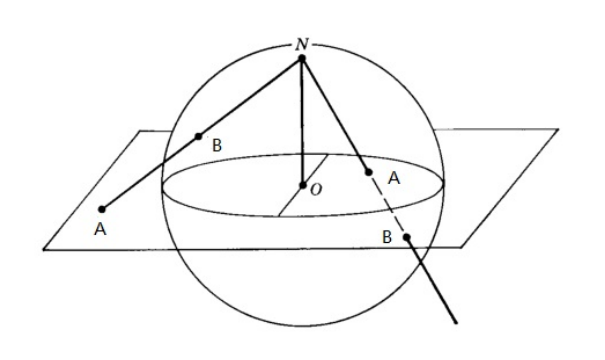
\includegraphics[width=0.5\textwidth]{p75}
    \caption{stereographic projection from north pole to plane $z = 0$.}
    \label{fig:plot_1}
\end{figure}
\begin{enumerate}[label=(\alph*)]
    \item For $A = (x,y,z), N = (0,0,1)$ in above plot\footnote{Picture source: \url{http://pi.math.cornell.edu/~boyang/2220\%20s2017/math2220_notes/notes_sec_2.1.pdf}}, then $\overrightarrow{NA} = (x,y,z-1)$. The stereographic projection of $A$ can be set by $B = (x',y',0)$, then $\overrightarrow{BN} = (x',y',-1)$. Also, $\overrightarrow{NA}$ is parallel to $\overrightarrow{NB}$, which gives $\overrightarrow{NA} = k \overrightarrow{NB}$. Then,
    \begin{align*}
        x' = \frac{x}{1-z},\quad y' = \frac{y}{1-z}.
    \end{align*}
    Thus,
    \begin{align*}
        \pi_N(x,y,z) = \left(\frac{x}{1-z}, \frac{y}{1-z}\right).
    \end{align*}
    
    \item Suppose $B = (u,v,0)$, and we want to know the coordinates of $A$. $\overrightarrow{NB} = (u,v,-1)$ and then $\overrightarrow{NA} = k \overrightarrow{NB} = (ku,kv,-k)$, which gives the coordinates of $A = (ku, kv, 1-k)$. Also, $A$ is on the unit ball. Then,
    \begin{align*}
        (ku)^2 + (kv)^2 + (1-k)^2 = 1,
    \end{align*}
    which implies $k = \frac{2}{u^2 + v^2 + 1}$. Thus, 
    \begin{align*}
        \pi^{-1}_N(u,v) = \left(\frac{2u}{u^2+v^2+1}, \frac{2v}{u^2+v^2+1}, \frac{u^2+v^2-1}{u^2+v^2+1}\right).
    \end{align*}
    
    \item \begin{enumerate}[label=\arabic*)]
        \item If $\pi^{-1}_N(u_1,v_1) = \pi^{-1}_N(u_2, v_2)$, then
        \begin{align*}
            \frac{2u_1}{u_1^2+v_1^2+1} = \frac{2u_2}{u_2^2+v_2^2+1},\quad \frac{2v_1}{u_1^2+v_1^2+1} = \frac{2v_2}{u_2^2+v_2^2+1},
        \end{align*}
        which implies $u_1/v_1 = u_2/v_2$, and similarly, we have
        \begin{align*}
            u_1^2+v_1^2-1 = u_2^2+v_2^2-1.
        \end{align*}
        Then, $u_1 = u_2, v_1 = v_2$. Thus, $\pi^{-1}_N$ is one-to-one and hence $\pi^{-1}_N$ is immersion.
        
        \item For any $(x,y,z) \in S^2 \setminus \{N\}$, there exists a point $\left(\frac{x}{1-z}, \frac{y}{1-z}\right)$ such that 
        \begin{align*}
            \pi^{-1}_N \left(\frac{x}{1-z}, \frac{y}{1-z}\right) = (x,y,z).
        \end{align*}
        Thus, $\pi^{-1}_N$ is onto, and hence it is homeomorphism.
    \end{enumerate}
\end{enumerate}
\end{proof}


\medskip

\begin{problem}
Prove that the tangent space\footnote{Suppose $G$ is a subspace of $GL(n, \mathbb{R})$; that is, $G$ is a group of $n \times n$ matrices. The {\em tangent space at the identity} of $G$ is the set of all matrices having the form $f'(0)$, for some function $f: \mathbb{R} \to G$, which is differentiable at $t = 0$ and satisfies $f(0) = I_n$. Definition source: \url{https://www.mtholyoke.edu/courses/hpollats/M319ps6_07.pdf}.} to $O(3)$ at the identity matrix $I \in O(3)$ has the following description:
$$T_I O(3)=\{A\in \mathbb{R}^{3\times 3}:\, A+A^T=0\}.$$
\end{problem}
\begin{proof}
If $A \in T_I O(n)$, then there is a path $B(t)$ in orthogonal group $O(n)$ with $B(0) = I$ and $DB(0) = A$, where $B^T(t)B(t) = I$\cite{3}. Taking derivative on both sides with respect to $t$ gives 
\begin{align*}
    0 = DB(0)^T \cdot I + I \cdot DB(0) = A^T + A.
\end{align*}
\end{proof}


\medskip


\noindent
{\bf Problem 77.}
If $f$ is continuous, show that
$$
\int_0^x\int_0^y\int_0^z f(t)\, dt\, dz\, dy =
\frac{1}{2}\int_0^x (x-t)^2f(t)\, dt.
$$

\begin{proof}

\end{proof}


\medskip

\noindent
{\bf Problem 78.}
 Prove that $\mathbb{R}^n\subset\mathbb{R}^{n+1}$ embedded as the plane generated by the
first $n$ coordinates has ($(n+1)$-dimensional) measure zero.
\begin{proof}
	WRITE YOUR SOLUTION HERE.
\end{proof}


\medskip

\noindent
{\bf Problem 79.}
Prove that the standard ternary Cantor set has measure zero.
\begin{proof}
	WRITE YOUR SOLUTION HERE.
\end{proof}


\medskip

\noindent
{\bf Problem 80.}
Prove that if $f:[0,1]\to [0,1]$ is a continuous function then its graph as
a subset of $\mathbb{R}^2$ has measure zero.
\begin{proof}
Since $f$ is continuous on a compact set, then $f$ is uniformly continuous, i.e., for any $\varepsilon > 0$, there exists $\delta > 0$, such that if $|x - y| < \delta$, then $|f(x) - f(y)| \leq \varepsilon/2$. Now let $\delta = 1/n$ for some $n$ such that above condition holds. Denote the set $\left[f\left(k/n\right), f\left((k+1)/n\right)\right] \times \left[f\left(k/n\right) - \frac{\varepsilon}{2}, f\left(k/n\right) + \frac{\varepsilon}{2}\right]$ by $P_k, k = 0,1,\cdots,n-1$\, then the volume $|P_k| = \frac{\varepsilon}{n}$. Then, the graph $G_f$ of $f$ satisfies $G_f \subset \bigcup^n_{k=1} P_k$ and then 
\begin{align*}
    |G_f| = \sum^n_{i=1} |P_k| = n \frac{\varepsilon}{n} = \varepsilon \to 0.
\end{align*}
Thus, the graph of $f$ has measure zero.
\end{proof}


\medskip

\noindent
{\bf Problem 81.}
Prove that if $f:\mathbb{R}^n\to\mathbb{R}^n$ is a Lipschitz function, i.e.
$|f(x)-f(y)|\leq L|x-y|$ for all $x,y\in\mathbb{R}^n$ and some $L>0$ and
$E\subset\mathbb{R}^n$ is a set of measure zero, then $f(E)\subset\mathbb{R}^n$
has measure zero.
\begin{proof}
For any $\varepsilon > 0$, since $E$ has measure zero, then let $E \subset \cup^\infty_{i=1} B(x_i, r_i)$, where $\sum^\infty_{i=1} r_i^n < \varepsilon/L^n$. 

Since $f$ is Lipschitz function, then $f \left(B(x_i, r_i)\right) \subset B \left(f(x_i), Lr_i)\right)$. Indeed, for $x \in B(x_i, r_i)$,
\begin{align*}
    |f(x) - f(x_i)| < L|x - x_i| < Lr_i,
\end{align*}
and then $f(x) \in B \left(f(x_i), Lr_i)\right)$. Now we have 
\begin{align*}
    f(E) \subset \bigcup^\infty_{i=1} f\left(B(x_i, r_i)\right) \subset \bigcup^\infty_{i=1} B \left(f(x_i), Lr_i)\right),
\end{align*}
and thus
\begin{align*}
    |f(E)| \leq \sum^\infty_{i=1} (Lr_i)^n < \varepsilon,
\end{align*}
which implies $f(E)$ has measure zero.
\end{proof}


\medskip

\noindent
{\bf Problem 82.}
Let $f:\mathbb{R}^3\to\mathbb{R}^2$ be a continuous function. Let $K\subset\mathbb{R}^3$ be a compact set such that $|f(x)-f(y)|\leq 2012|x-y|^{2}$
for all $x,y\in K$. Prove that the set $f(K)\subset\mathbb{R}^2$ has measure zero as a subset of $\mathbb{R}^2$.
\begin{proof}
We do not assume $K$ has measure zero. Since $K$ is compact, then there exists $M > 0$ such that $K \subset [-M,M]^3$ and $K$ can be covered by $n^3$ closed cubes $Q_i$ of side-length $2M/n$, whose diameter is $2\sqrt{3}M/n$. Each such cube can be covered by a closed ball of radius $2\sqrt{3}M/n$ centered at any point of the cube. Then, $K$ can be covered by no more than $n^3$ balls $B\left(x_i, 2\sqrt{3}M/n\right), x_i \in K$, such that $Q_i \cap K \neq \varnothing$ and $Q_i \cap K \subset B\left(x_i, 2\sqrt{3}M/n\right)$. Now, 
\begin{align*}
    f\left( B\left(x_i, 2\sqrt{3}M/n\right)\right) \subset B \left(f(x_i), 2012 \left(2\sqrt{3}M/n\right)^2 \right),
\end{align*}
also, $K \subset \bigcup^k_i B\left(x_i, 2\sqrt{3}M/n\right)$, $k \leq n^3$, then,
\begin{align*}
    f(K) \subset \bigcup^k_i B \left(f(x_i), 2012 \left(2\sqrt{3}M/n\right)^2 \right).
\end{align*}
Denote $2012 \left(2\sqrt{3}M/n\right)^2$ by $r_i$, then
\begin{align*}
    \sum^k_{i=1} r_i^2 \leq c n^{-4} n^3 = c n^{-1} \xrightarrow[]{n\to\infty} 0.
\end{align*}
Thus, $f(K)$ has measure zero.
\end{proof}



\medskip

\noindent
{\bf Problem 83.}
Assume that $f : [0, 1]\to [0, 1]$ is a continuous function such that the set
$\{x\in [0, 1] :\,  f(x) = 1\}$ has measure zero. Prove directly (without using any results like monotone or
dominated convergence theorem) that
$$
\lim_{n\to\infty} \int_0^1 f(x)^n\, dx =0.
$$
\begin{proof}
Let $E = \{x \in [0,1] | f(x) = 1\}$. For fixed $\varepsilon > 0$, since $E$ has zero measure, then $E \subset \bigcup^k_{i=1}I_i$, where $I_i$ are open and $\sum^k_{i=1}|I_i| < \varepsilon/2$, i.e., $\bigcup^k_{i=1}I_i$ are a covering of $E$ by open intervals of total lengths less than $\varepsilon/2$. 

By compactness of $[0,1]$, $[0,1]\setminus \bigcup^k_{i=1}I_i$ is closed and hence compact. Then $f$ attains maximum $M$ on this set, which is strictly less than $1$, and hence $|f(x)| \leq M < 1$ for all $x \in [0,1]\setminus \bigcup^k_{i=1}I_i$. Then,
\begin{align*}
    f(x) \leq \begin{cases}
        1, & x \in \bigcup^k_{i=1}I_i, \\
        M^n, & x \notin \bigcup^k_{i=1}I_i.
    \end{cases}
\end{align*}
and then we have
\begin{align*}
    \int^1_0 f^n\, dx & \leq 1 \cdot \left|\sum^k_{i=1} I_i \right| + M^n \cdot 1, \\
    & \leq \frac{\varepsilon}{2} + M^n.
\end{align*}
Since $M < 1$, then there exists $N > 0$ such that for all $n \geq N$, $M^n < \varepsilon/2$. Thus, for all $n \geq N$, $\int^1_0 f^n\, dx \leq \varepsilon \to 0$.
\end{proof}


\medskip

\noindent
{\bf Problem 84.}
Let $f:[0,1]\to (0,\infty)$ be a $C^1$ function. Find a diffeomorphism
of $(0,1)\times(0,1)$ onto the domain
$\{ (x,y): x\in (0,1),\, 0<y<f(x)\}$. Then apply the change of variables
formula to this diffeomorphism to show that the area under the graph of $f$ equals
$\int_0^1 f(x)\, dx$.
\begin{proof}
	WRITE YOUR SOLUTION HERE.
\end{proof}


\medskip

\noindent
{\bf Problem 85.}
The mapping $\Phi:\mathbb{R}^2\to (0,\infty)\times (-\infty,0)$,
$\Phi(x,y)=(e^x,-e^y)$ is a diffeomorphism (take it for granted; do not prove it).
Let $g:[1,e]\times [-e,-1]\to\mathbb{R}$
be continuous. Express the integral
$$
\int_1^e\int_{-e}^{-1} g(x,y)\, dx\, dy
$$
using $\Phi$ as a change of variables (Just write the integral. It is impossible to evaluate
it, because we do not know the function $g$.).
\begin{proof}
	WRITE YOUR SOLUTION HERE.
\end{proof}


\medskip

\noindent
{\bf Problem 86.}\\
{\bf (a)}
Let $\varphi_i=\varphi_i(x_1,x_2,\ldots,x_i):\mathbb{R}^i\to\mathbb{R}$
be $C^1$ functions for $i=1,2\ldots, n-1$.
Prove that the mapping
$\Phi:\mathbb{R}^n\to\mathbb{R}^n$ defined by
$$
\Phi(x_1,x_2,\ldots,x_n) =
(x_1,\varphi_1(x_1)+2x_2, \varphi_2(x_1,x_2)+3x_3,\ldots,
\varphi_{n-1}(x_1,x_2,\ldots,x_{n-1})+nx_n)
$$
is a diffeomorphism onto an open subset of $\mathbb{R}^n$.\\
{\bf (b)} Find the volume of $\Phi((0,1)^n)$, where $(0,1)^n$
is an open unit cube in $\mathbb{R}^n$.
\begin{proof}
	WRITE YOUR SOLUTION HERE.
\end{proof}



\medskip


\noindent
{\bf Problem 87.}
Let $\gamma:\mathbb{R}\to\mathbb{R}^n$ and $\mathbf{v}_i:\mathbb{R}\to\mathbb{R}^n$, $i=1,2,\ldots,n-1$, be $C^\infty$ smooth functions such that
for any $t\in\mathbb{R}$ the vectors
$$
\gamma'(t),\mathbf{v}_1(t),\ldots,\mathbf{v}_{n-1}(t)
$$
form an orthonormal basis of $\mathbb{R}^n$ (here we differentiate $\gamma$ but {\bf do not} differentiate $\mathbf{v}_i$, $i=1,2,\ldots,n-1$).

Consider the mapping $\Phi:\mathbb{R}^n\to\mathbb{R}^n$ defined by
$$
\Phi(x_1,\ldots,x_n)=\gamma(x_n)+\sum_{i=1}^{n-1} x_i\mathbf{v}_i(x_n).
$$
\begin{itemize}
	\item[(a)] Find the derivative $D\Phi(x_1,\ldots,x_n)$;
	\item[(b)] Prove that $\Phi$ is a diffeomorphism in a neighborhood of a point of the form $(0,\ldots,0,x_n)$;
	\item[(c)] Find the limit
	$$
	\lim_{r\to 0}
	\frac{|\Phi(B^n(0,r))|}{|B^n(0,r)|}\, ,
	$$
	where $B^n(0,r)$ denotes the ball of radius $r$ centered at the origin and $|A|$ stands for the volume of the set $A$.
\end{itemize}
\begin{proof}
~\begin{enumerate}[label=(\alph*)]
    \item 
    \begin{align*}
        D\Phi(x_1,\cdots,x_n) = \begin{pmatrix}
            \mathbf{v}_1(x_n) &  &  &  &  \\
            & \mathbf{v}_2(x_n) &  &  &  \\
            &  & \ddots &  & \\
            &  &  & \mathbf{v}_{n-1}(x_n) \\
            &  &  &  & \gamma'(x_n) + \sum^{n-1}_{i=1}x_i \mathbf{v}_i'(x_n)
        \end{pmatrix}.
    \end{align*}
    
    \item 
    \begin{align*}
        D\Phi(0,\ldots, 0, x_n) = \begin{pmatrix}
            \mathbf{v}_1(x_n) &  &  &  &  \\
            & \mathbf{v}_2(x_n) &  &  &  \\
            &  & \ddots &  & \\
            &  &  & \mathbf{v}_{n-1}(x_n) \\
            &  &  &  & \gamma'(x_n)
        \end{pmatrix}.
    \end{align*}
    is an orthogonal matrix and then $\det D\Phi(0,\ldots, 0, x_n) = \pm 1 \neq 0$. Then it remains to show that $\Phi$ is bijection. And this is obvious. Thus, $\Phi$ is a diffeomorphism in a neighborhood of a point of the form $(0,\ldots,0,x_n)$.
    
    \item By the change of variable, we have
    \begin{align*}
        \left|\Phi(B^n(0,r))\right| = \int_{B^n(0,r)} |J_\Phi|\, dA
    \end{align*}
    and $|J_\Phi| \to 1$ as $r \to 0$, Then for any $\varepsilon > 0$, there exists $r$ such that $\left||J_\Phi| - 1\right| < \varepsilon$, and then
    \begin{align*}
        \left|\frac{|\Phi(B^n(0,r))|}{|B^n(0,r)|} - 1\right| = \left|\frac{\int_{B^n(0,r)} |J_\Phi|\, dA}{|B^n(0,r)|} - 1\right|< \varepsilon.
    \end{align*}
    Thus, the limit is equal to $1$.
\end{enumerate}
\end{proof}


\medskip

\noindent
{\bf Problem 88.}
Let $\Phi:\mathbb{R}^2\to\Phi(\mathbb{R}^2)\subset\mathbb{R}^2$ be a diffeomorphism. Prove that
$$
\int_{B^2(0,1)}\Vert D\Phi\Vert  =\int_{\Phi(B^2(0,1))}\Vert D(\Phi^{-1})\Vert,
$$
where $\Vert A\Vert=(\sum_{i,j=1}^2 a_{ij}^2)^{1/2}$ is the Hilbert-Schmidt norm of the matrix.\\
{\bf Hint.} {\em Compare $\Vert A\Vert$ and $\Vert A^{-1}\Vert$ for a $2\times 2$ matrix.}
\begin{proof}
For $A = \begin{pmatrix} 
    a & b \\
    c & d
\end{pmatrix}$, we have $\|A\| = \left(a^2 + b^2 + c^2 + d^2\right)^{1/2}$, then $A^{-1} = \frac{1}{ad - bc}\begin{pmatrix} 
    d & -b \\
    -c & a
\end{pmatrix}$ and thus $\left\|A^{-1}\right\| = \frac{\left(a^2 + b^2 + c^2 + d^2\right)^{1/2}}{ad - bc}$. 

Now we consider $\Phi: \mathbb{R}^2 \to \Phi\left(\mathbb{R}^2\right) \subset \mathbb{R}^2$, and for $x \in \mathbb{R}^2$, there exists $y \in \mathbb{R}^2$, $\Phi(x) = y$. Then, with 
\begin{align*}
    \int_{B^2(0,1)} (f \circ \Phi)\left|J_\Phi\right| = \int_{\Phi\left(B^2(0,1)\right)} f,
\end{align*}
taking $f = \left\|D\left(\Phi^{-1}\right) \right\|$ gives
\begin{align*}
    \int_{\Phi\left(B^2(0,1)\right)} \left\|D\left(\Phi^{-1}\right) \right\| = \int_{B^2(0,1)} \left\|D\left(\Phi^{-1}\right) (\Phi(x)) \right\| \cdot \left|J_\Phi\right|.
\end{align*}

Then it suffices to show that
\begin{align*}
    \left\|D\left(\Phi^{-1}\right) (\Phi(x)) \right\| \cdot \left|J_\Phi(x)\right| = \left\|D\Phi(x) \right\|.
\end{align*}
Also, we have $\Phi^{-1} \circ \Phi = I$\footnote{Here $I$ means identity map, like $f(x) = x, x \in \mathbb{R}^n$. Hence, the derivative of $\Phi^{-1} \circ \Phi$ is identity.}, then $D\left(\Phi^{-1}\right)(\Phi(x)) D\Phi(x) = I$. Then,
\begin{align*}
    D\left(\Phi^{-1}\right)(\Phi(x)) = \left(D\Phi(x)\right)^{-1},
\end{align*}
and then multiplying both sides by $\left|J_\Phi\right|$ gives
\begin{align*}
    \left\|D\left(\Phi^{-1}\right) (\Phi(x)) \right\| \cdot \left|J_\Phi(x)\right| = \left\|\left(D\Phi(x)\right)^{-1} \right\| \left|J_\Phi(x)\right|.
\end{align*}

Then it remains to show that 
\begin{align*}
    \left\|\left(D\Phi(x)\right)^{-1} \right\| \left|J_\Phi(x)\right| = \left\|D\Phi(x) \right\|.
\end{align*}
With above results, we have $\left\|A^{-1}\right\| |\det A|= \|A\|$, and the above equality follows.
\end{proof}

\medskip

\noindent
{\bf Problem 89.}
Prove that if $K\in C^1(\mathbb{R}^2\setminus
\{ (0,0)\})$ satisfies the estimate
$$
|\nabla K(x)|\leq \frac{1}{|x|^3} \quad \mbox{for all $x\neq (0,0)$}
$$
then there is a constant $C>0$ such that
$$
\iint_{\{x\in\mathbb{R}^2:\, |x|>2|y|\}} |K(x-y)-K(x)|\, dx\leq C
$$
for all $y\in\mathbb{R}^2$.\\
{\bf Hint:} {\em Use the mean value theorem to estimate
	$|K(x-y)-K(x)|$ and then integrate in polar coordinates.}
\begin{proof}
Denote the left hand side by $I$. If $y = 0$, then $I = 0$. We can assume $|y| > 0$, and the point of interval connecting $x$ to $x - y$ are of form $x - ty, t \in [0,1]$. Then, with $|x| > 2|y|$,
\begin{align*}
    |x - ty| > |x| - |y| > \frac{|x|}{2}.
\end{align*}
With mean value theorem, 
\begin{align*}
    |K(x-y) - K(x)| & \leq |\nabla K(x-ty)| \cdot |(x - y) - x| \\
    & \leq \frac{|y|}{|x-ty|^3} \\
    & \leq \frac{8|y|}{|x|^3}.
\end{align*}
Thus,
\begin{align*}
    \iint_{|x|>2|y|} |K(x-y)-K(x)|\, dx & \leq \iint_{|x|>2|y|} \frac{8|y|}{|x|^3}\, dx \\
    & = 8|y| \int^{2\pi}_0 \int^\infty_{2|y|} \frac{1}{r^3}r\, dr d\theta \\
    & = 8|y| 2\pi \left(- r^{-1}\right)\Big|_{2|y|}^\infty = 8 \pi.
\end{align*}
\end{proof}


\medskip


\noindent
{\bf Problem 90.}
Prove that
$$
\int_0^1\int_0^1 \frac{1}{1-xy}\, dx\, dy =\sum_{n=1}^\infty \frac{1}{n^2}
$$
The integral is understood as an improper integral
$\displaystyle\lim_{t\to 1^-} \int_0^t\int_0^t\ldots$.
\begin{proof}
Define
\begin{align*}
    I_t = \int^t_0 \int^t_0 \frac{1}{1 - xy}\, dx dy = \int^t_0 \int^t_0 \sum^\infty_{n=0} (xy)^n \, dx dy = \int^t_0 \left(\int^t_0 \sum^\infty_{n=0} x^n y^n \, dx \right)dy,
\end{align*}
Also, since
\begin{align*}
    \sum^\infty_{n=0} \left|x^n y^n \right| = \sum^\infty_{n=0} x^n y^n \leq \sum^\infty_{n=0} t^{2n} = \frac{1}{1 - t^2},
\end{align*}
$\sum^\infty_{n=0} x^n y^n$ converges uniformly on $[0,t]$. Hence, 
\begin{align*}
    I_t & = \int^t_0 \left(\sum^\infty_{n=0} \int^t_0 x^ny^n \, dx \right)dy = \int^t_0 \sum^\infty_{n=0} \left(\frac{x^{n+1}}{n+1}y^n \right)\Bigg|^t_{x=0} dy \\
    & = \int^t_0 \sum^\infty_{n=0} \frac{t^{n+1}}{n+1}y^n dy.
\end{align*}
Similarly, $\sum^\infty_{n=0} \frac{t^{n+1}}{n+1}y^n$ converges uniformly on $[0,t]$, and hence
\begin{align*}
    I_t & = \sum^\infty_{n=0} \int^t_0 \frac{t^{n+1}}{n+1}y^n dy = \sum^\infty_{n=0} \frac{t^{n+1}}{n+1} \left(\frac{y^{n+1}}{n+1}\right)\Bigg|^t_0 \\
    & = \sum^\infty_{n=0} \left(\frac{t^{n+1}}{n+1}\right)^2 \xlongequal{m=n+1} \sum^\infty_{m=1}\frac{t^{2m}}{m^2} \xrightarrow[t\to 1^-]{\clubsuit} \sum^\infty_{m=1} \frac{1}{m^2}.
\end{align*}
Proof of $\clubsuit$:
\begin{align*}
    \left| \sum^\infty_{m=1} \frac{1}{m^2} - \sum^\infty_{m=1} \frac{1-t^{2m}}{m^2} \right| = \sum^k_{m=1} \frac{1 - t^{2m}}{m^2} + \sum^\infty_{m=k+1} \frac{1 - t^{2m}}{m^2}
\end{align*}
For $\forall \varepsilon > 0$, there exists $k > 0$ such that \begin{align*}
    \sum^\infty_{m=k+1} \frac{1 - t^{2m}}{m^2} \leq \sum^\infty_{m=k+1} \frac{1}{m^2} < \frac{\varepsilon}{2},
\end{align*}
also, there exists $t_0$ such that for $t_0 < t < 1$, 
\begin{align*}
    \sum^k_{m=1} \frac{1 - t^{2m}}{m^2} < \frac{\varepsilon}{2}.
\end{align*}
Thus, for $\varepsilon > 0$, 
\begin{align*}
    \left| \sum^\infty_{m=1} \frac{1}{m^2} - \sum^\infty_{m=1} \frac{1-t^{2m}}{m^2} \right| < \varepsilon.
\end{align*}
\end{proof}


\medskip


\noindent
{\bf Problem 91.}
Suppose that $f:\mathbb{R}^2\to [0,\infty)$ is uniformly continuous on $\mathbb{R}^2$ and
$$
\sup_{r>0} \iint_{\{x^2+y^2\leq r^2\}} f(x,y)\, dxdy <\infty.
$$
Prove that $\displaystyle \lim_{|(x,y)|\to\infty} f(x,y)=0$.
\begin{proof}
	WRITE YOUR SOLUTION HERE.
\end{proof}


\medskip

\noindent
{\bf Problem 92.}
Use Green's theorem to prove the following result:
If the vertices of a polygon, in counterclockwise order, are
$(x_1,y_1)$, $(x_2,y_2)$, \ldots,$(x_n,y_n)$, then the area of the
polygon is
$$
A=\frac{1}{2}
\sum_{i=1}^n(x_iy_{i+1}-x_{i+1}y_i),
$$
where we use notation $x_{n+1}=x_1$, $y_{n+1}=y_1$.
\begin{proof}
By Green's theorem, the area is
\begin{align*}
    A = \frac{1}{2} \int_C x\, dy - y\, dx = \frac{1}{2} \sum^n_{i=1} \int^{(x_{i+1}, y_{i+1})}_{(x_{i}, y_{i})} x\, dy - y\, dx.
\end{align*}
Let $\alpha(t) = \left(x_i + t(x_{i+1} - x_{i}), y_i + t(y_{i+1} - y_{i}) \right), t\in [0,1]$ is a parameterization of the segment connecting $(x_{i}, y_{i})$ to $(x_{i+1}, y_{i+1})$. Let $\gamma(t) = (x(t), y(t)) \to \mathbb{R}^2, t \in [a,b]$, then 
\begin{align*}
    \int_\gamma P\, dx + Q\, dy = \int^b_a \left(P(x(t),y(t))x'(t) + Q(x(t),y(t))y'(t) \right)\, dt
\end{align*}
Then,
\begin{align*}
    \int^{(x_{i+1}, y_{i+1})}_{(x_{i}, y_{i})} x\, dy - y\, dx & = \int^1_0 (x_i + t(x_{i+1} - x_{i}))(y_{i+1} - y_i) - (y_i + t(y_{i+1} - y_{i}))(x_{i+1} - x_i)\, dt \\
    & = \left(tx_i + \frac{t^2}{2}(x_{i+1} - x_i)\right) (y_{i+1} - y_i)\Bigg|^1_0 \\
    & - \left(ty_i + \frac{t^2}{2} (y_{i+1} - y_i)\right) (x_{i+1} - x_i)\Bigg|^1_0 \\
    & = x_i y_{i+1} - x_{i+1} y_i,
\end{align*}
and hence,
\begin{align*}
    A = \frac{1}{2} \sum_{i=1}^n (x_i y_{i+1} - x_{i+1} y_i).
\end{align*}
\end{proof}


\medskip

\noindent
{\bf Problem 93.}
Let $\Omega\subset\mathbb{R}^2$ be a bounded
domain with $C^1$ boundary and let $\Phi:\mathbb{R}^2\to\mathbb{R}^2$,
$\Phi(x,y)=(u(x,y), v(x,y))$,
be a
$C^2$ diffeomorphism. Prove that
$$
\int_{\partial\Omega} uv_x\, dx + uv_y\, dy = \pm|\Phi(\Omega)|\, ,
$$
where $|\Phi(\Omega)|$ denotes the area of $\Phi(\Omega)$
and $\partial\Omega$ has positive orientation.
Show on examples that both cases $+|\Phi(\Omega)|$ and
$-|\Phi(\Omega)|$ are possible.

\begin{proof}
By Green's theorem, $\int_{\partial \Omega} P\, dx + Q\, dy = \iint_D \frac{\partial Q}{\partial x} - \frac{\partial P}{\partial y}$, then
\begin{align*}
    \int_{\partial\Omega} uv_x\, dx + uv_y\, dy & = \iint_\Omega \frac{\partial}{\partial x} \left(uv_y \right) - \frac{\partial}{\partial y} \left(uv_x \right) \\
    & = \iint_\Omega u_xv_y + u v_{yx} - u_y v_x - u v_{xy} \\
    & = \iint_\Omega u_xv_y - u_y v_x,
\end{align*}
where in the last step we used the fact that $\Phi \in C^2$. Moreover, 
\begin{align*}
    \iint_\Omega u_xv_y - u_y v_x = \iint_\Omega \begin{vmatrix}
        u_x & u_y \\
        v_x & v_y
    \end{vmatrix} = \iint_\Omega \det D\Phi.
\end{align*}
In particular, with change of variable, we have
\begin{align*}
    \int_{\Phi(\Omega)} f = \int_{\Omega} (f\circ \Phi) |\det D\Phi|,
\end{align*}
setting $f = 1$ gives
\begin{align*}
    \int_{\Omega} |\det D\Phi| = |\Phi(\Omega)|.
\end{align*}
Thus, 
\begin{align*}
    \int_{\partial\Omega} uv_x\, dx + uv_y\, dy = 
    \begin{cases}
        |\Phi(\Omega)|, & \det D\Phi > 0, \\
        - |\Phi(\Omega)|, & \det D\Phi < 0.
    \end{cases}
\end{align*}

Taking $\Phi(x,y) = (x,y)$, then the integral equals to $|\Phi(\Omega)|$, if we take $\Phi(x,y) = (-x,y)$, then the integral equals to $-|\Phi(\Omega)|$.
\end{proof}


\medskip




\noindent
{\bf Problem 94.}
Suppose that $f\in C^2(\mathbb{R}^3)$ is constant in a neighborhood of the boundary of
a ball $B\subset\mathbb{R}^3$. Prove that
$$
\iiint_B (f_{xx}+f_{yy}+f_{zz})\, dV = 0\, .
$$
\begin{proof}
	WRITE YOUR SOLUTION HERE.
\end{proof}


\medskip

\noindent
{\bf Problem 95.}
Let $D =\{(x, y)\in\mathbb{R}^2 : x^2 + y^2\leq 1\}$ and $f\in C^\infty(\mathbb{R}^2)$. Suppose that $f(x, y) = 1$ for all
$(x, y)\in\partial D$. Prove that
$$
\iint_D \left(2f(x,y)+x\frac{\partial f}{\partial x}+y\frac{\partial f}{\partial y}\right)dA=2\pi.
$$
\begin{proof}
By Green's theorem, $\int_{\partial \Omega} P\, dx + Q\, dy = \iint_D \frac{\partial Q}{\partial x} - \frac{\partial P}{\partial y}$, then the area of $D$ is 
\begin{align*}
    A = \frac{1}{2} \int_{\partial D} x\, dy - y\, dx.
\end{align*}
Indeed, 
\begin{align*}
    \frac{1}{2} \int_{\partial D} x\, dy - y\, dx = \frac{1}{2} \iint_D 2\, dA = A.
\end{align*}

Now let $P = -yf, Q = xf$, then 
\begin{align*}
    \frac{\partial Q}{\partial x} - \frac{\partial P}{\partial y} = 2f + x \frac{\partial f}{\partial x} + y \frac{\partial f}{\partial y},
\end{align*}
and thus
\begin{align*}
    \iint_D \left(2f(x,y)+x\frac{\partial f}{\partial x}+y\frac{\partial f}{\partial y}\right)\, dA & = \int_{\partial D} -yf\, dx + x f\, dy \\
    & = \int_{\partial D} -y \, dx + x \, dy \\
    & = \iint_D 2\, dA = 2\pi.
\end{align*}
\end{proof}


\medskip


\noindent
{\bf Problem 96.}
Let $x = (x_1, x_2)$  and $f(x) $ be a $C^2$ function on $\mathbb{R}^2$ such that
$ |\partial^2 f (x)/\partial x_j \partial x_k| \le 1$ for all $x \in \mathbb{R}^2$ and $ j, k \in \{1,2\}$.
Prove that
$$
\bigg|\iint_{|x| \le 1} f(x) dA - \pi f(0,0)\bigg| \le 3/2.
$$
\begin{proof}
	WRITE YOUR SOLUTION HERE.
\end{proof}


\medskip



\noindent
{\bf Problem 97.}
Suppose $f(x,y)$ is a $C^2$ function on the unit disk $\mathbb{D} = \{(x,y)\,|\,x^2+y^2\leq 1\}$ such that for some $M>0$ and all $(x,y)\in\mathbb{D}$,
$$ \left[f_{xx}(x,y)\right]^2 + 2\left[f_{xy}(x,y)\right]^2 + \left[f_{yy}(x,y)\right]^2 \leq M. $$
If $f(0,0) = f_x(0,0) = f_y(0,0) = 0$, show that
$$ \left\lvert \iint_{\mathbb{D}} f(x,y)\,\mathit{dx}\mathit{dy} \right\rvert \leq \frac{\pi\sqrt{M}}{4} $$
\begin{proof}
	WRITE YOUR SOLUTION HERE.
\end{proof}


\medskip


\noindent
{\bf Problem 98.}
Let $f$ be a polynomial of total degree at most three in $(x, y, z) \in \mathbb{R}^3$.  Prove that:
$$
\int_{x^2 + y^2 + z^2 \le 1} f(x, y, z)\hspace{1.5pt} dx\hspace{1.5pt}  dy \hspace{1.5pt} dz =
\frac{4\pi f((0, 0, 0)) }{3} +  \frac{2\pi \left(\Delta f\right)((0, 0, 0))}{15}.
$$
Here $\displaystyle{\Delta =  \frac{\partial^2}{\partial x^2}  +  \frac{\partial^2}{\partial y^2} +
	\frac{\partial^2}{\partial z^2}}$ is the Laplacian operator on $\mathbb{R}^3$.
\begin{proof}
With Taylor's formula, 
\begin{align*}
    f(x) = f(0) + \sum^3_{i=1} \frac{\partial f}{\partial x_i}(0) x_i + \frac{1}{2} \sum^3_{i,j=1} \frac{\partial^2 f}{\partial x_i \partial x_i}(0)x_i x_i + \frac{1}{6} \sum^3_{i,j,k=1} \frac{\partial^3 f}{\partial x_i \partial x_i \partial x_k}(0)x_i x_i x_k + R.
\end{align*}
and since $f$ is a polynomial of degree at most $3$, then the remainder $R = 0$. Also, with the property of odd function,
\begin{align*}
    \int_B x_i\, dx = 0,\quad \int_B x_i x_i x_k\, dx = 0,
\end{align*}
and
\begin{align*}
    \int_B x_i x_i\, dx = 0,\,\, i\neq j.
\end{align*}
Then, 
\begin{align*}
    \int_B f(x, y, z)\, dx\,dy\,dz = f(0) \underbrace{\int_B\, dx}_{4\pi/3}  + \frac{1}{2} \sum^3_{i=1} \frac{\partial^2 f}{\partial x^2_i}(0) \int_B x_i^2\, dx,
\end{align*}
also, with 
\begin{align*}
    \int_B x_1^2\, dx = \int_B x_2^2\, dx = \int_B x_3^2\, dx & = \frac{1}{3} \int_B |x|^2\, dx \\
    & = \int^1_0 \int_{S(r)} r^2\, d\sigma\, dr \\
    & = \int^1_0 r^2 \cdot 4\pi r^2\, dr = \frac{4\pi}{5},
\end{align*}
the proof is completed. 
\end{proof}


\medskip

\noindent
{\bf Problem 99.}
Suppose that $K\in C^\infty(\mathbb{R}^2\setminus \{ 0\})$ and
$$
K(x)=\frac{K(x/\Vert x\Vert)}{\Vert x\Vert}
\quad
\text{for all $x\in\mathbb{R}^2\setminus\{0\}$.}
$$
\begin{itemize}
	\item[(a)] Prove that $\nabla K(tx)=t^{-2}\nabla K(x)$ for $x\neq 0$ and $t>0$.
	\item[(b)] Use the divergence theorem to prove that (on both sides we integrate vector valued functions)
	$$
	\int_{\{1\leq \Vert x\Vert\leq 2019\}} \nabla K(x)\, dx=
	\int_{\partial \{1\leq \Vert x\Vert\leq 2019\}} K(x)\vec{\mathbf{n}}\, d\sigma(x).
	$$
	\item[(c)] Prove that
	$$
	\int_{\{1\leq \Vert x\Vert\leq 2019\}} \nabla K(x)\, dx=0.
	$$
\end{itemize}
{\bf Hint.} {\em Show first that
	$K(tx)=t^{-1}K(x)$ for $x\neq 0$, $t>0$. In (a) differentiate $K(tx)$. Part (a) is not needed for parts (b) and (c).}
\begin{proof}
~\begin{enumerate}[label=(\alph*)]
    \item Note that 
    \begin{align*}
        K(tx) = \frac{K(tx/\Vert tx\Vert)}{\Vert tx\Vert} = t^{-1} \frac{K(x/\Vert x\Vert)}{\Vert x\Vert} = t^{-1} K(x).
    \end{align*}
    Then, 
    \begin{align*}
        t^{-1} \frac{\partial K}{\partial x_i}(x) = \frac{\partial }{\partial x_i}(t^{-1} K(x)) = \frac{\partial }{\partial x_i}(K(tx)) = \frac{\partial K}{\partial x_i}(tx) \cdot t,
    \end{align*}
    which gives,
    \begin{align*}
        \frac{\partial K}{\partial x_i}(tx) = t^{-2} \frac{\partial K}{\partial x_i}(x).
    \end{align*}
    Thus,
    \begin{align*}
        \nabla K(tx) = t^{-2} \nabla K(x).
    \end{align*}
    
    \item With divergence theorem, $\int_\Omega \div \vec{F} = \int_{\partial \Omega} \vec{F}\cdot \vec{\mathbf{n}}$, if $F(x) = (K(x), 0)$, then $\div F = \frac{\partial K}{\partial x_1}$ and then
    \begin{align*}
        \int_{\{1\leq \Vert x \Vert\leq 2019\}} \frac{\partial K}{\partial x_1} = \int_{\partial\{1\leq \Vert x \Vert\leq 2019\}} F \cdot \vec{\mathbf{n}} \, d\sigma(x) = \int_{\partial\{1\leq \Vert x \Vert\leq 2019\}} K(x) n_1 \, d\sigma(x),
    \end{align*}
    where in the last step we used $F \cdot \vec{\mathbf{n}} = (K(x), 0)\cdot (n_1, n_2) = K(x) n_1$.
    
    
    Similarly, if $F(x) = (0,K(x))$, then $\div F = \frac{\partial K}{\partial x_2}$ and then
    \begin{align*}
        \int_{\{1\leq \Vert x \Vert\leq 2019\}} \frac{\partial K}{\partial x_2} = \int_{\partial\{1\leq \Vert x \Vert\leq 2019\}} K(x) n_2 \, d\sigma(x).
    \end{align*}
    Thus, 
    \begin{align*}
        \int_{\{1\leq \Vert x\Vert\leq 2019\}} \nabla K(x)\, dx = \int_{\partial \{1\leq \Vert x\Vert\leq 2019\}} K(x)\vec{\mathbf{n}}\, d\sigma(x).
    \end{align*}
    
    \item 
    \begin{align*}
        \int_{\{1\leq \Vert x\Vert\leq 2019\}} \nabla K(x)\, dx & = \int_{\partial \{1\leq \Vert x\Vert\leq 2019\}} K(x)\vec{\mathbf{n}}\, d\sigma(x) \\
        & = - \int_{\Vert x\Vert = 1} K(x) \frac{x}{\Vert x\Vert}\, d\sigma(x) + \int_{\Vert x\Vert = 2019} K(x) \frac{x}{\Vert x\Vert}\, d\sigma(x).
    \end{align*}
    Note that $K(2019 x) = 2019^{-1} K(x)$. Use standard parameterization of the circle, we have
    \begin{align*}
        \int_{\gamma} f\, dx dy = \int^b_a f(x(t), y(t)) \sqrt{\Dot{x}(t)^2 + \Dot{y}(t)^2} \, dt,
    \end{align*}
    where $\gamma: [a,b] \to \mathbb{R}$ and $|\Dot{\gamma}(t)| = \sqrt{\Dot{x}(t)^2 + \Dot{y}(t)^2}$. Take $\gamma(t) = 2019 (\cos t, \sin t)$, then 
    \begin{align*}
        \int_{\Vert x\Vert = 2019} K(x) \frac{x}{\Vert x\Vert}\, d\sigma(x) & = \int^{2\pi}_0 K(2019 \cos t, 2019 \sin t) \frac{(2019 \cos t, 2019 \sin t)}{2019} 2019 \, dt \\
        & = \int^{2\pi}_0 K(\cos t, \sin t) \frac{(\cos t, \sin t)}{1} \, dt \\
        & = \int_{\Vert x\Vert = 1} K(x) \frac{x}{\Vert x\Vert}\, d\sigma(x).
    \end{align*}
    Thus, 
    \begin{align*}
        \int_{\{1\leq \Vert x\Vert\leq 2019\}} \nabla K(x)\, dx = 0.
    \end{align*}
\end{enumerate}
\end{proof}


\medskip


\noindent
{\bf Problem 100.}
 For $x=(x_1,x_2)\in\mathbb{R}^2$, let $|x|=\sqrt{x_1^2+x_2^2}$.
Let $D=\{x\in\mathbb{R}^2:\, |x|< 1\}$ and let $f:\overline{D}\to\mathbb{R}$ be continuous on $\overline{D}$. Prove that
$$
\lim_{n\to\infty} \iint_D (n+2)|x|^n f(x)\, dA=\int_0^{2\pi} f(\cos t,\sin t)\, dt.
$$
\begin{proof}
	WRITE YOUR SOLUTION HERE.
\end{proof}

\newpage
\bibliographystyle{unsrt}
\bibliography{bibliography}

\end{document}